%-------------------------------------------------------------------------------------------------------------------------------------------
%	PACKAGES AND OTHER DOCUMENT CONFIGURATIONS
%-------------------------------------------------------------------------------------------------------------------------------------------

\documentclass[a4paper,11pt]{article} % Font and paper size
\linespread{0.9}
%----------------------------------------------------------------------------------------
%	PACKAGES AND OTHER DOCUMENT CONFIGURATIONS
%----------------------------------------------------------------------------------------

\usepackage[utf8]{inputenc} % Required for inputting international characters
\usepackage[T1]{fontenc} % Output font encoding for international characters
\usepackage[italian]{babel} % Italian dictionary


\usepackage[table]{xcolor} % Required for custom colors
\usepackage{gensymb}
\usepackage{amsmath}
\usepackage{bm}
\usepackage{tikz}
\usepackage{hhline}
\usepackage{listings}
\usepackage{enumitem}

%\usepackage[margin=2cm, includefoot]{geometry} % Modify margins
\usepackage{fancyhdr}
\usepackage{rotating}
\usepackage[hidelinks]{hyperref} % Hyperlinks

\usepackage[none]{hyphenat}% Non spezza le parole nelle tabelle
\usepackage{array}

\usepackage{graphicx} % Required for figures
\usepackage{float}
\usepackage{wrapfig}
\usepackage{caption}
\usepackage{subcaption}

%pagestyle
\pagestyle{fancy}
\fancyhead{}
\fancyfoot{}
\fancyfoot[R]{\thepage}
\renewcommand{\headrulewidth}{0pt}



\usepackage{xfrac}
\usepackage{amssymb}

\usepackage{multicol}
\usepackage{multirow}

\usepackage[toc, page]{appendix}
\usepackage{booktabs}
\usepackage{siunitx}


%----------------------------------------------------------------------------------------
%	NEW COMMANDS
%----------------------------------------------------------------------------------------

\newcommand{\restr}[2]{{% we make the whole thing an ordinary symbol
\left.\kern-\nulldelimiterspace % automatically resize the bar with \right
#1 % the function

\right|_{#2} % this is the delimiter
}}

\newcommand{\tnhl}{\tabularnewline\hline}
\newcommand{\tn}{\tabularnewline}
\newcolumntype{x}[1]{%
	>{\centering\hspace{0pt}}p{#1}}%


 % Include the file specifying document layout and packages
\usepackage{pifont}
\newcommand{\cmark}{\ding{51}}%
\newcommand{\xmark}{\ding{55}}%
\usepackage{titlesec}
\titlespacing{\section}{0em}{1em}{0.5em}
\titlespacing{\subsection}{0em}{1em}{0.5em}
\setlength{\parindent}{0pt}

%-------------------------------------------------------------------------------------------------------------------------------------------
%	GENERAL INFORMATION 
%-------------------------------------------------------------------------------------------------------------------------------------------

\newcommand{\labcourse}{Laboratorio di Fisica}
\newcommand{\teacher}{Docenti: Prof. A. Garfagnini - Prof. M. Lunardon}
\newcommand{\laurea}{Corso di Laurea in Fisica}
\newcommand{\channel}{Canale 1 A-L}
\newcommand{\academicyear}{Anno Accademico 2020/2021}
\newcommand{\labexp}{Esperienza di Laboratorio}
\newcommand{\exptitle}{Catena Elettronica}
\newcommand{\turno}{Turno T2}
\newcommand{\name}{Nicolò Lai}
\newcommand{\matricola}{1193976}
\newcommand{\mail}{nicolo.lai@studenti.unipd.it}
\newcommand{\consegna}{Data Esperienza}
\newcommand{\data}{23/11/2020 \\ 25/11/2020 \\ 26/11/2020}


%-------------------------------------------------------------------------------------------------------------------------------------------
%	DOCUMENT 
%-------------------------------------------------------------------------------------------------------------------------------------------

\begin{document}
%\sloppy

%-------------------------------------------------------------------------------------------------------------------------------------------
%	REFERNCE CUSTOMIZATION
%-------------------------------------------------------------------------------------------------------------------------------------------

\def\sectionautorefname{Sezione} 
\def\subsectionautorefname{Sezione} 
\def\subsubsectionautorefname{Sezione}

\abovedisplayshortskip=0pt
\belowdisplayshortskip=0pt
\abovedisplayskip=-5pt
\belowdisplayskip=5pt

%-------------------------------------------------------------------------------------------------------------------------------------------
%	TITLE PAGE
%-------------------------------------------------------------------------------------------------------------------------------------------

\begin{titlepage}
	\begin{center}
		\Huge{\bfseries \labcourse}\\
			
		\LARGE \teacher \\
		\Large \laurea\\
		\Large \channel\\
		\Large \academicyear\\
		[1cm] 
		\line(1,0){400}\\
		[3.5cm]
			
		\textsc{\huge{\bfseries \labexp}}\\
		\huge{\exptitle}\\
		[2mm] \line(1,0){300}\\
		[9cm]
	\end{center}
	
	
	\begin{flushleft}
		\textsc{\Large \turno}\\
		[0.5cm] \textsc{\large {\bfseries \name}} \\ 
		\indent\large \matricola \\ 
		\indent\large \mail \\
	\end{flushleft}
		
					
	\begin{flushright}
			\textsc{\Large\consegna}\\
			\textsc{\large \data}					
	\end{flushright}
			
\end{titlepage}
\cleardoublepage


%-------------------------------------------------------------------------------------------------------------------------------------------
%	OBIETTIVO
%-------------------------------------------------------------------------------------------------------------------------------------------

\section{Obiettivo}

Assemblare una catena elettronica associata ad un rivelatore di radiazione. Studiare il segnale in uscita e la risposta
in frequenza dei singoli moduli e della catena elettronica completa.


%-------------------------------------------------------------------------------------------------------------------------------------------
%	APPARATO SPERIMENTALE
%-------------------------------------------------------------------------------------------------------------------------------------------

\section{Strumentazione e Componenti}\label{s:strumenti}

Nel corso dell'esperienza vengono utilizzati:
\begin{itemize}[itemsep=-0.5ex]
	\item Multimetro digitale Metrix MTX3292
	\item Generatore di funzioni Tektronix AFG1022
	\item Oscilloscopio digitale Tektronix TBS1102B
	\item Alimentatore di tensione continua TTi
	\item Due circuiti integrati TL082C (in totale quattro amplificatori operazionali)
	\item Resistori e condensatori di varie taglie
	\item Scheda Arduino Due
\end{itemize}


%-------------------------------------------------------------------------------------------------------------------------------------------
%	CATENA ELETTRONICA
%-------------------------------------------------------------------------------------------------------------------------------------------

\section{Introduzione}\label{s:intro}

L'esperienza si basa su l'assemblamento e sullo studio della risposta di una serie di moduli volti a simulare
l'elettronica associata ad un \textit{rivelatore di radiazione}. In laboratorio, quindi, si utilizza il generatore di
funzioni per simulare un segnale acquisibile dalla rivelazione di un evento da parte del detector. Questo segnale viene
inizialmente elaborato dal \textit{preamplificatore} (di tipo \textit{charge sensitive}) e successivamente dallo
\textit{shaper} (di tipo \textit{CR-RC}). Il segnale in uscita dal formatore viene infine amplificato per favorirne
l'acquisizione da parte di una DAQ, che corrisponde in questo caso all'ADC della scheda Arduino Due. I tre stadi
(\textit{preamplificatore}, \textit{shaper}, \textit{amplificatore}) costituiscono dunque la \textit{catena elettronica}
rappresentata in \autoref{i:circuito}.

\begin{figure}[H]
	\centering
	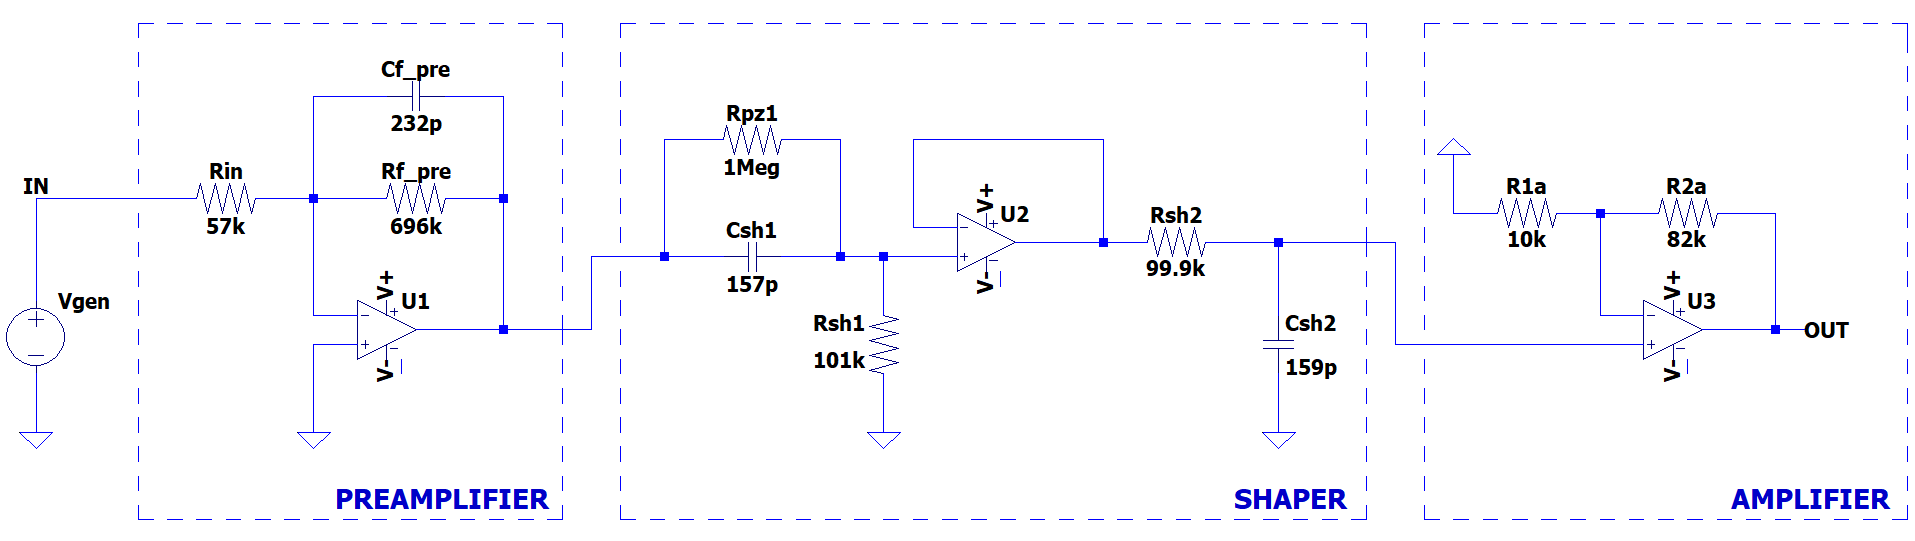
\includegraphics[width=0.9\linewidth]{../Simulations/catena_circuito.png}
	\caption{\small Schema a costanti concentrate della catena elettronica suddivisa nei tre moduli di interesse.}
	\label{i:circuito}
\end{figure}


%-------------------------------------------------------------------------------------------------------------------------------------------
%	PREAMPLIFICATORE
%-------------------------------------------------------------------------------------------------------------------------------------------

\section{Preamplificatore}\label{s:preamp} 

Il primo stadio della catena \textit{(preamplificatore)} si utilizza per migliorare il rapporto segnale/rumore, in modo
da trasferire un segnale più pulito all'elettronica di acquisizione. In laboratorio si assembla un preamplificatore
\textit{charge sensitive}: il modulo, infatti, consiste di un circuito integratore e la tensione in uscita è quindi
direttamente proporzionale alla carica in ingresso. Nelle sezioni successive si vuole ricavare analiticamente il
comportamento teorico del preamplificatore e, successivamente, verificarne l'accordo con la risposta sperimentale. In
particolare, ci si concentra sulle caratteristiche del segnale in uscita, la sua linearità rispetto alla carica in
ingresso e sull'analisi in frequenza del circuito.


%-------------------------------------------------------------------------------------------------------------------------------------------
%	CONFIGURAZIONE SPERIMENTALE
%-------------------------------------------------------------------------------------------------------------------------------------------

\subsection{Configurazione Sperimentale}\label{s:preamp_config}

Si comincia utilizzando il generatore per simulare i segnali del rivelatore, impostando sul CH1 un impulso quadrato di
frequenza $f_{\text{gen}} = 1 \,\si{k\Hz}$, tensione di riferimento $V_{\text{high}} = 0 \,\si{\volt}$, ampiezza
\textit{negativa} $V_{\text{low}} = -1 \,\si{\volt}$ e durata $T = 5 \,\si{\us}$ (cioè il tempo di raccolta del
segnale). Viene successivamente assemblato sulla breadboard il primo modulo in \autoref{i:circuito} utilizzando le
componenti circuitali riportate in \autoref{t:direct_measures}, misurate con il multimetro Metrix. È dunque fondamentale
che il segnale erogato dal generatore sia 

\begin{wraptable}{L}{0.5\textwidth}
	\small
	\centering
	\begin{tabular}{x{1.8cm} x{2.5cm} x{2cm} } \toprule[0.5px]\toprule[0.1px]	
		\multicolumn{3}{c}{Misure Dirette - Preamplificatore}\tn
		\midrule[0.1px]
		Label & Valore & F.S. \tn
		\addlinespace
		$R_{\text{in}}$ & $56.56 \pm 0.02\,\si{k\ohm}$ & $100\,\si{k\ohm}$ \tn
		$R_{\text{f}}$ & $696.1 \pm 0.3\,\si{k\ohm}$ & $1000\,\si{k\ohm}$ \tn
		$C_{\text{f}}$ & $232 \pm 9\,\si{p\farad}$ & $1000\,\si{p\farad}$ \tn
		\bottomrule[0.5px]		
	\end{tabular}
	\caption{\small Misure dirette delle componenti circuitali.}
	\label{t:direct_measures}
\end{wraptable}	

\textit{negativo}: avendo un amplificatore operazionale in configurazione \textit{invertente} è infatti una richiesta
necessaria per poter avere in output un segnale positivo, cioè già acquisibile con la scheda Arduino Due. Si utilizza
poi un generatore di tensione continua con $V_{\text{cc}} = +15 \,\si{\volt}$ e $V_{\text{ee}} = -15 \,\si{\volt}$ per
alimentare l'operazionale. Si assume che esso abbia un comportamento ideale, ovvero che il polo positivo ed il polo
negativo si trovino allo stesso potenziale (\textit{virtual short}). Il segnale in ingresso $V_{\text{in}}$ viene
prelevato nel punto \textit{IN} evidenziato nello schema mentre il segnale in uscita $V^{\text{pre}}_{\text{out}}$ dal
preamplificatore viene prelevato al termine del primo modulo, entrambi utilizzando sonde 10X.


%-------------------------------------------------------------------------------------------------------------------------------------------
%	TRATTAZIONE ANALITICA
%-------------------------------------------------------------------------------------------------------------------------------------------

\subsection{Trattazione Analitica}\label{s:preamp_th} 

Concentrando inizialmente l'attenzione sul modulo di ingresso (generatore reale e cablaggio), il sistema è un filtro
passa basso con frequenza di taglio $f_{\text{t}}^{\text{in}}\approx 32 \,\si{\MHz}$, molto maggiore delle frequenze in
gioco: risulta allora corretto assumere il modulo in ingresso del tutto equivalente ad un generatore ideale, come
rappresentato in \autoref{i:circuito}. Trattando ora il preamplificatore, invece, la funzione di trasferimento del
circuito è riportata in \autoref{e:preamp_H}: si noti il segno negativo dovuto all'amplificatore operazionale posto in
configurazione invertente, la presenza di un unico polo e l'assenza di zeri. 

\begin{align}\label{e:preamp_H} 
	H(s) &= - \frac{ 1 }{ R_{\text{in}}\,C_{\text{f}} } \,\, \frac{1}{ s + \frac{1}{\tau_{\text{pre}} } } 
	& 
	&\text{con} \,\, \tau_{\text{pre}} = R_{\text{f}}\,C_{\text{f}}
\end{align} 

Data la forma della funzione di trasferimento, la risposta in frequenza sarà quella di un filtro \textit{passa basso}:
rappresentando $H(s)$ in un grafico di Bode ci si aspetta allora un andamento costante a basse frequenze fino alla
\textit{frequenza di taglio} $f_{\text{t}}=\frac{1}{2\pi\tau_{\text{pre}}}$ e una decrescita lineare con pendenza
$-20\,\text{dB/dec}$ per frequenze maggiori. Facendo riferimento ai valori delle componenti circuitali riportati in
\autoref{t:direct_measures}, il tempo caratteristico del preamplificatore e la frequenza di taglio del filtro risultano
essere

\begin{align}\label{e:preamp_stime_th}
	\tau_{\text{pre}} & = 161 \pm 6 \,\si{\us}
	&
	f_{\text{t}} & = 0.99 \pm 0.04 \,\si{\kilo\Hz}
\end{align}

Si ricava, infine, la risposta del circuito ad un segnale a gradino: nell'approssimazione $T\ll\tau_{\text{pre}}$ si trova
una crescita lineare direttamente proporzionale alla carica in ingresso al preamplificatore per $0 < t < T$ e una
decrescita smorzata esponenzialmente per $t \gg T$:

\begin{align}\label{e:preamp_vout} 
	V^{\text{pre}}_{\text{out}}(t) &= \begin{cases} -\frac{ Q_{\text{in}}
	(t)}{C_{\text{f}} } & 0 < t < T \\
        -\frac{ Q_{\text{c}} }{ C_{\text{f}} } \, e^{ -\frac{ t }{ \tau^{\text{pre}} } } & t \gg T \\
    \end{cases}
    & 
    &\text{con} \,\,\, 
    \begin{cases} 
        Q_{\text{in}} (t) = I_{\text{in}}\,t = \frac{ V_{\text{in}} }{ R_{\text{in}} }\,t \\
        Q_{\text{c}} = I_{\text{in}}\,T = \frac{ V_{\text{in}} }{ R_{\text{in}} }\,T \\
    \end{cases}
\end{align} 

dove, appunto, $Q_{\text{in}} (t)$ corrisponde alla carica raccolta al tempo $t$ dal preamplificatore mentre
$Q_{\text{c}}$ rappresenta la carica \textit{totale} accumulata nel preamplificatore. Ci si aspetta allora che il
segnale in uscita $V_{\text{out}}$ visualizzato sull'oscilloscopio presenti una salita lineare fino ad un valore di
tensione massimo $V_{\text{out}}^{\text{max}} = \frac{Q_{\text{c}}}{C_{\text{f}}}$ e, successivamente, una decrescita
esponenziale di tempo caratteristico $\tau_{\text{pre}}$. \\

Al fine di verificare il corretto funzionamento dell'apparato sperimentale, si riportano in \autoref{t:preamp_sper_th}
le misure sperimentali del massimo della tensione e della costante di tempo $\tau_{\text{pre}}$ acquisite con
l'oscilloscopio. 

\begin{wraptable}{R}{0.50\textwidth}
	\small
	\centering
	\begin{tabular}{x{1.8cm} x{1.8cm} x{1.7cm} x{1.7cm}} \toprule[0.5px]\toprule[0.1px]	

		\multicolumn{4}{c}{Controllo Apparato - Preamplificatore} \tn

		\midrule[0.1px]

		$V_{\text{max}}^{\text{th}} \,(\si{\milli\volt})$ & $V_{\text{max}}^{\text{sper}} \,(\si{\milli\volt})$ &
		$\tau_{\text{pre}}^{\text{th}} \,(\si{\us})$ & $\tau_{\text{pre}}^{\text{sper}} \,(\si{\us})$ \tn

		\addlinespace

		$388 \pm 17$ & $392 \pm 7$ & $161 \pm 6$ & $158 \pm 2$ \tn

		\bottomrule[0.5px]		
	\end{tabular}
	\caption{\small Confronto tra stime teoriche e misure sperimentali.}
	\label{t:preamp_sper_th}
\end{wraptable}	

Confrontando ultime con le aspettative teoriche si nota chiaramente come ci sia un accordo generale tra le predizioni
analitiche e l'effettiva risposta del preamplificatore. Osservando poi \autoref{e:preamp_vout}, è esplicita la
dipendenza lineare del segnale in uscita rispetto alla carica in ingresso al preamplificatore: nella sezione successiva
si vuole quindi verificare che tale linearità venga rispettata. Chiaramente, è importante che ciò avvenga in quanto la
carica in questione rappresenta in questo caso un'idealizzazione del rivelamento di radiazione ionizzante da parte di un
detector: è logico richiedere dunque che il preamplificatore risponda in modo lineare alla quantità di carica che riceve
in ingresso.


%-------------------------------------------------------------------------------------------------------------------------------------------
%	LINEARITA DEL PREAMP
%-------------------------------------------------------------------------------------------------------------------------------------------

\subsection{Linearità del Preamplificatore}\label{s:preamp_linearity}

Ci si propone ora di verificare la dipendenza lineare del segnale in uscita $V^{\text{pre}}_{\text{out}}$ dalla carica
in ingresso $Q_{\text{in}}$ come esposto in \autoref{e:preamp_vout}. Si fa variare dunque la durata $T$ del segnale
erogato dal generatore di funzioni da $2\,\si{\us}$ a $10\,\si{\us}$, in modo da modificare di volta in volta la
quantità di carica iniettata nel preamplificatore rimanendo nell'approssimazione $T\ll\tau_{\text{pre}}$: per ogni $T$
viene calcolata la quantità di carica totale $Q_{\text{c}}$ e viene misurato con l'oscilloscopio il valore massimo del
segnale in uscita $V^{\text{max}}_{\text{out}}$. Ai valori di tensione misurati con l'oscilloscopio viene associato
l'errore di acquisizione comprendente sia il contributo di lettura sia il contributo sul guadagno verticale in quanto
nel processo di misura sono state utilizzate scale diverse, con la consapevolezza che queste ultime portano ad una
correlazione almeno parziale delle incertezze. Gli errori sulla carica $Q_{\text{c}}$, invece, vengono calcolati per
propagazione assumendo, ragionevolmente, che l'incertezza sulla durata $T$ del segnale sia trascurabile. Questi
risultano allora totalmente correlati tra loro: $V_{\text{in}}$ e $R_{\text{in}}$ rimangono costanti e l'incertezza
sulla carica è dunque semplicemente l'incertezza sulla corrente in ingresso al preamplificatore riscalata dal tempo $T$.


\begin{wraptable}{L}{0.50\textwidth}

	\small
	\centering

	\begin{tabular}{x{1.5cm} x{2.5cm} x{2.5cm}} 
		
		\toprule[0.5px]\toprule[0.1px]	

		\multicolumn{3}{c}{Linearità del Preamplificatore - Misure}\tn

		\midrule[0.1px]

		$T\,(\si{\us})$ & $Q_{\text{c}}\,(\si{\pico\coulomb})$ & $V^{\text{max}}_{\text{out}}\,(\si{\milli\volt})$ \tn

		\addlinespace

		$2 $	&	$36.0	\pm 0.7$	&	$162	\pm 3 $ \tn
		$3 $	&	$54.0	\pm 1.0$	&	$238	\pm 4 $ \tn
		$4 $	&	$72.0	\pm 1.3$	&	$320	\pm 6 $ \tn
		$5 $	&	$90		\pm 2  $	&	$392	\pm 7 $ \tn
		$6 $	&	$108	\pm 2  $	&	$472	\pm 8 $ \tn
		$7 $	&	$126	\pm 2  $	&	$548	\pm 9 $ \tn
		$8 $	&	$144	\pm 3  $	&	$632	\pm 12$ \tn
		$9 $	&	$162	\pm 3  $	&	$704	\pm 13$ \tn
		$10$	&	$180	\pm 3  $	&	$776	\pm 14$ \tn
		
		\bottomrule[0.5px]

	\end{tabular}

	\caption{\small Dati relativi al grafico in \autoref{i:preamp_linearity}.}

	\label{t:preamp_data}

\end{wraptable}	

Si rappresentano ora in \autoref{i:preamp_linearity} le coppie $\{Q_{\text{c}},\,V^{\text{max}}_{\text{out}}\}$: il
coefficiente angolare della retta di regressione corrisponde analiticamente all'inverso della capacità di feedback
$C_{\text{f}}$. Si vuole evidenziare che gli errori relativi su $V^{\text{pre}}_{\text{out}}$ e su $Q_{\text{c}}$ sono
entrambi circa il $2\%$ della misura: nell'effettuare la regressione si decide tuttavia di trascurare l'incertezza sulla
carica $Q_{\text{c}}$ (in quanto totalmente correlata) e di aggiungere tale contributo successivamente nel calcolo
dell'errore sulla capacità $C_{\text{f}}$ in \autoref{e:preamp_cf}. La bontà del fit, l'andamento dei residui, l'errore
a posteriori ed il confronto di $C_{\text{f}}^{\text{fit}}$ con quanto misurato direttamente con il multimetro verranno
presi in considerazione per verificare la linearità del preamplificatore rispetto alla carica in ingresso. 

\begin{figure}[H]
	\centering
	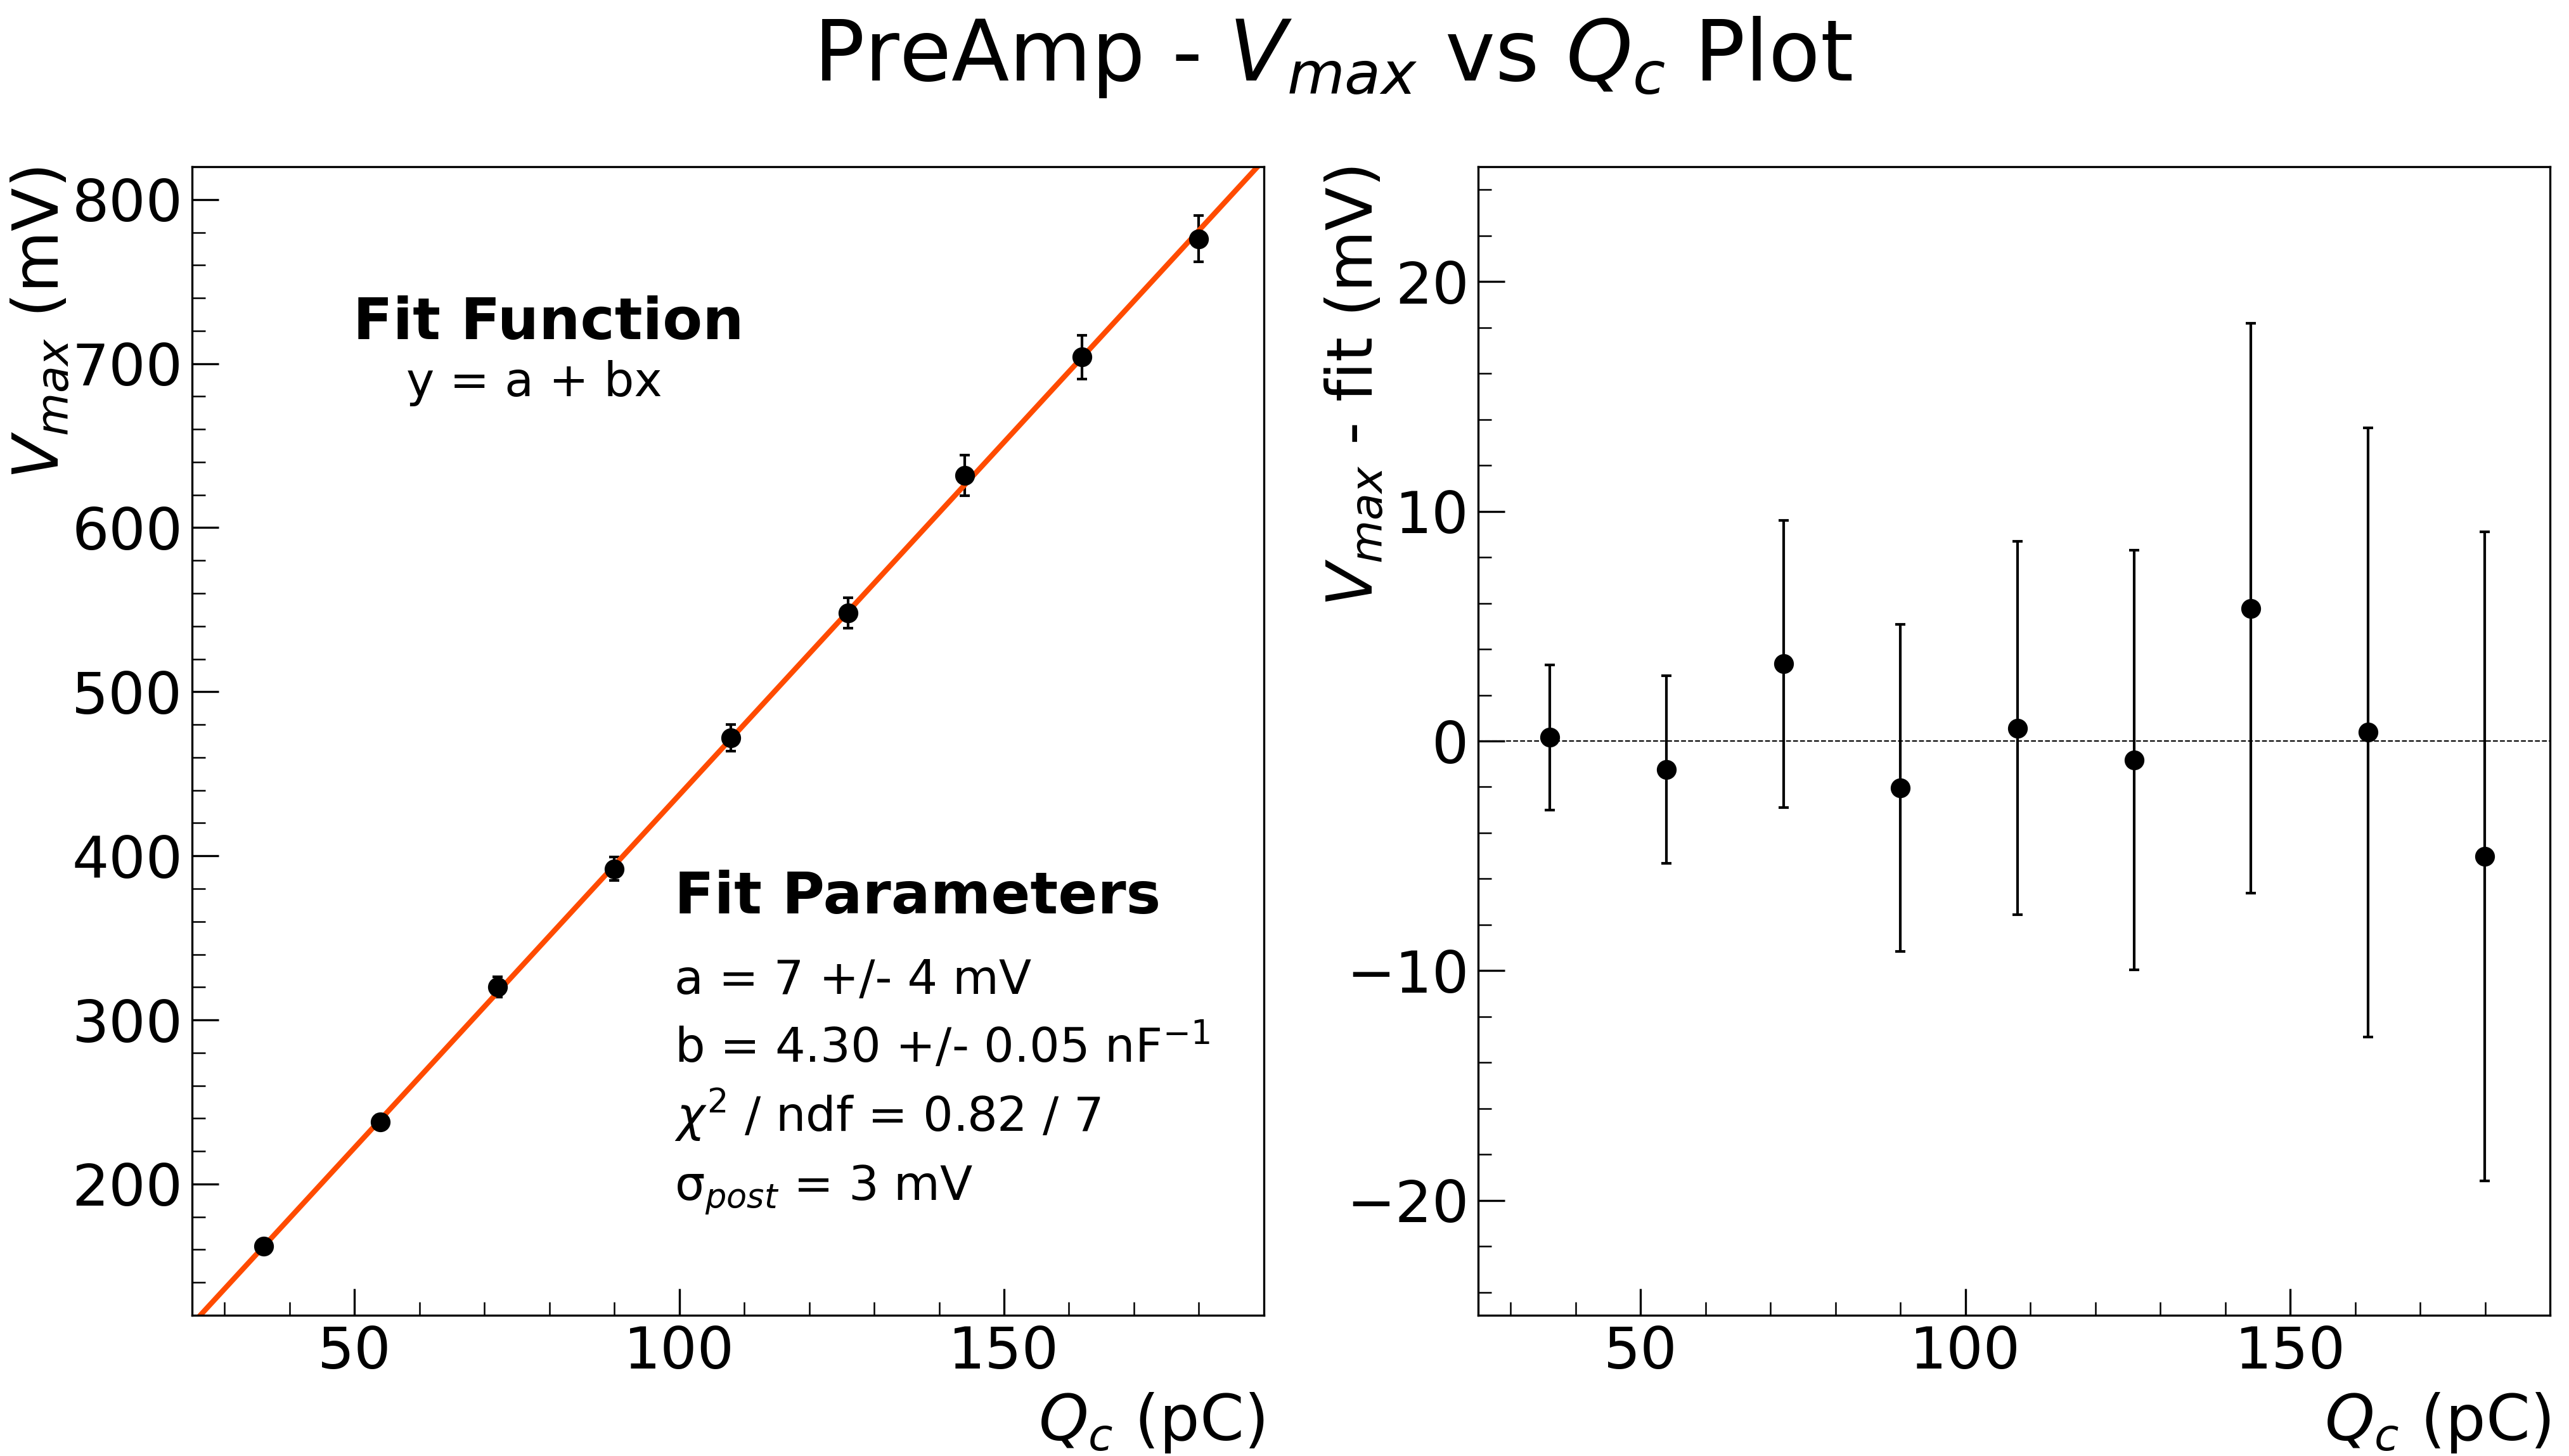
\includegraphics[width=0.9\linewidth]{../Plots/PreAmp/linearity_fit.png}
	\caption{\small Fit lineare del massimo di tensione in uscita contro la carica totale in ingresso.}
	\label{i:preamp_linearity}
\end{figure}

Si noti, inizialmente, come il $\chi^2$ della regressione sia notevolmente inferiore rispetto al suo valore di
aspettazione: essendo a conoscenza della parziale correlazione tra gli errori di scala dell'oscilloscopio ciò non
risulta essere sorprendente in quanto il fit non ne tiene ovviamente conto. Segue direttamente una sottostima
dell'errore sui parametri $a$ e $b$ della retta del fit. Un piccolo valore di $\chi^2$ rispetto al numero di gradi di
libertà, purtroppo, non permette nè di confermare l'ipotesi di linearità né di poterla rigettare. L'errore a posteriori,
invece, si trova essere dello stesso ordine di grandezza dell'errore associato alle tensioni più basse (i primi punti)
mentre diventa gradualmente inferiore rispetto all'incertezza associata alle tensioni maggiori. Questo suggerisce una
soddisfacente distribuzione dei punti attorno alla retta di regressione, che si traduce nel grafico dei residui in
un'ottimale distribuzione attorno allo zero. I residui, infatti, non presentano andamenti patologici accentuati e lo
zero risulta essere sempre ben compreso nelle barre d'errore. Concentrando ora l'attenzione sui parametri della retta
restituiti dal fit, si può notare come l'intercetta $a$ sia ben compatibile con zero, evidenziando l'assenza di un
eventuale offset sistematico o un errore di zero. Dal coefficiente angolare $b$ si ricava la stima della capacità

\begin{align}\label{e:preamp_cf}
	C_{\text{f}}^{\text{fit}}& = 232 \pm 7 \,\si{p\farad} 
	& 
	&\text{con} \,\,\,\, \sigma_{ C_{\text{f}}^{\text{fit}} } = 
	\sqrt
	{ 
		\left(
			\frac{1}{b^2}
		\right)^2
		\sigma_b^2 +
		2 \, \left(
			\frac{1}{b\,I}
		\right)^2
		\sigma_I^2
	}
\end{align}

dove, nel computo dell'errore, $\sigma_I$ rappresenta l'errore sulla corrente $I =
\frac{V_{\text{in}}}{R_{\text{in}}}$ che, nel fit, verrebbe riscalato dalla durata $T$ del segnale. La stima della
capacità di feedback risulta essere in ottima compatibilità ($\lambda = 0.05$) con quanto misurato con il multimetro
(\autoref{t:direct_measures}): questo porta quindi ad un'ulteriore conferma di una \textit{corretta} linearità del
preamplificatore.

%-------------------------------------------------------------------------------------------------------------------------------------------
%	SMORZAMENTO ESPONENZIALE
%-------------------------------------------------------------------------------------------------------------------------------------------

\subsection{Forma d'Onda del segnale in uscita}\label{s:preamp_waveform}

In questa sezione si vuole analizzare il segnale in uscita dal preamplificatore $V^{\text{pre}}_{\text{out}}$:
sfruttando la stessa configurazione sperimentale presentata in \autoref{s:preamp_config} viene acquisita la forma d'onda
del segnale utilizzando la scheda Arduino Due. Inizialmente allora si vogliono convertire le grandezze acquisite dalla
scheda in unità arbitrarie a grandezze fisicamente rilevanti. In particolare, dividendo il numero di acquisizione per il
sampling rate $S=0.955\,\text{Msps}$ si ottiene l'evoluzione temporale (in secondi) del segnale acquisito. Sfruttando
invece la funzione di calibrazione in tensione $V= a  +  b \cdot \text{counts}$ (con $a=-0.637 \pm 0.010\,\si{\volt}$ e
$b=0.828\pm0.007\,\si{mV/counts}$) si ottengono i valori in Volt delle misure acquisite in ADC counts. Per quanto
riguarda l'errore da associare a tali valori di tensione, ci si ritrova davanti ad un certo numero di complicazioni. La
prima idea sarebbe sfruttare gli errori sui parametri di calibrazione e, per propagazione, trovare l'incertezza sui
valori di tensione secondo 

\begin{equation}
	\sigma_{V} = \sqrt{\sigma_a^2 + \text{counts}^2 \cdot \sigma_b^2 + 2 \cdot \text{counts} \cdot \text{cov}(a,b)}
\end{equation}

Tuttavia, questa strategia porta ad una notevole sovrastima degli errori: così facendo, si associa ai valori di tensione
$V$ un'incertezza proveniente dal fit di calibrazione, pesato con gli errori di misura dati dall'oscilloscopio. Si perde
quindi l'informazione sull'accuratezza effettiva della scheda Arduino, che risulta essere invece decisamente migliore.
Inoltre, i parametri ($a$, $b$) e, soprattutto, i loro errori ($\sigma_a$, $\sigma_b$) della funzione di calibrazione
dipendono fortemente dal range di tensioni che si sceglie di adottare per la calibrazione: quest'ultima, infatti,
risulta essere sensibilmente differente per bassi valori di tensione (fino a circa $1.5\,\si{\volt}$) e per alti valori
di tensione a causa dei circuiti di protezione dei pin di ingresso. Si sceglie quindi di adottare una metodologia
differente per stimare le incertezze sui valori di tensione $V$. Ricordando che l'ADC della scheda Arduino Due converte
segnali analogici con tensione di riferimento $V_{\text{ref}}=3.3\,\si{\volt}$ su un range di $N = 12$ bit (ovvero 4096
valori), si trova una risoluzione di tensione dell’ADC, ovvero la più piccola variazione di tensione in ingresso che
causa la variazione di 1 bit del valore convertito in uscita, pari a 
\begin{equation}
	\Delta V = \frac{V_{\text{ref}}}{2^N} = \frac{3.3\,\si{\volt}}{4096} = 0.81 \,\si{\milli\volt}
\end{equation}\\
Per valutare gli effetti dell'accuratezza complessiva dell’acquisizione dell’ADC sulla stima della tensione in ingresso
ad Arduino, occorre ricordare che ciascun bit della conversione digitale ha un peso pari alla risoluzione di tensione
dell’ADC. Assumendo poi una un'accuratezza di $\pm 4$ LSB (bit meno significativo) sull’acquisizione dell’ADC si ottiene
un'accuratezza sulla stima della tensione in ingresso di $\Delta V \times 4 = 3.2 \,\si{\milli\volt}$. Assumendo infine
che questa si distribuisca uniformemente, si arriva alla stima finale dell'incertezza sulle stime dei valori di tensione
$\sigma_{V} = 1.9 \,\si{\milli\volt}$.\footnote{Tamberi, G. (2016). \textit{La Conversione Analogico/Digitale con
Arduino}. (Prima Edizione).} In \autoref{i:preamp_waveform} è esposto quanto acquisito dalla scheda Arduino: si nota
immediatamente come siano stati registrati due "eventi", o meglio nel tempo di acquisizione impostato per Arduino il
generatore di funzioni ha erogato due impulsi di tensione. Il segnale registrato, inoltre, risulta essere leggermente
rumoroso: per rendere l'analisi successiva meglio gestibile si decide di sovrapporre i due picchi di tensione e di
effettuarne una media. 

 \begin{wrapfigure}{R}{0.5\textwidth}
 	\centering
 	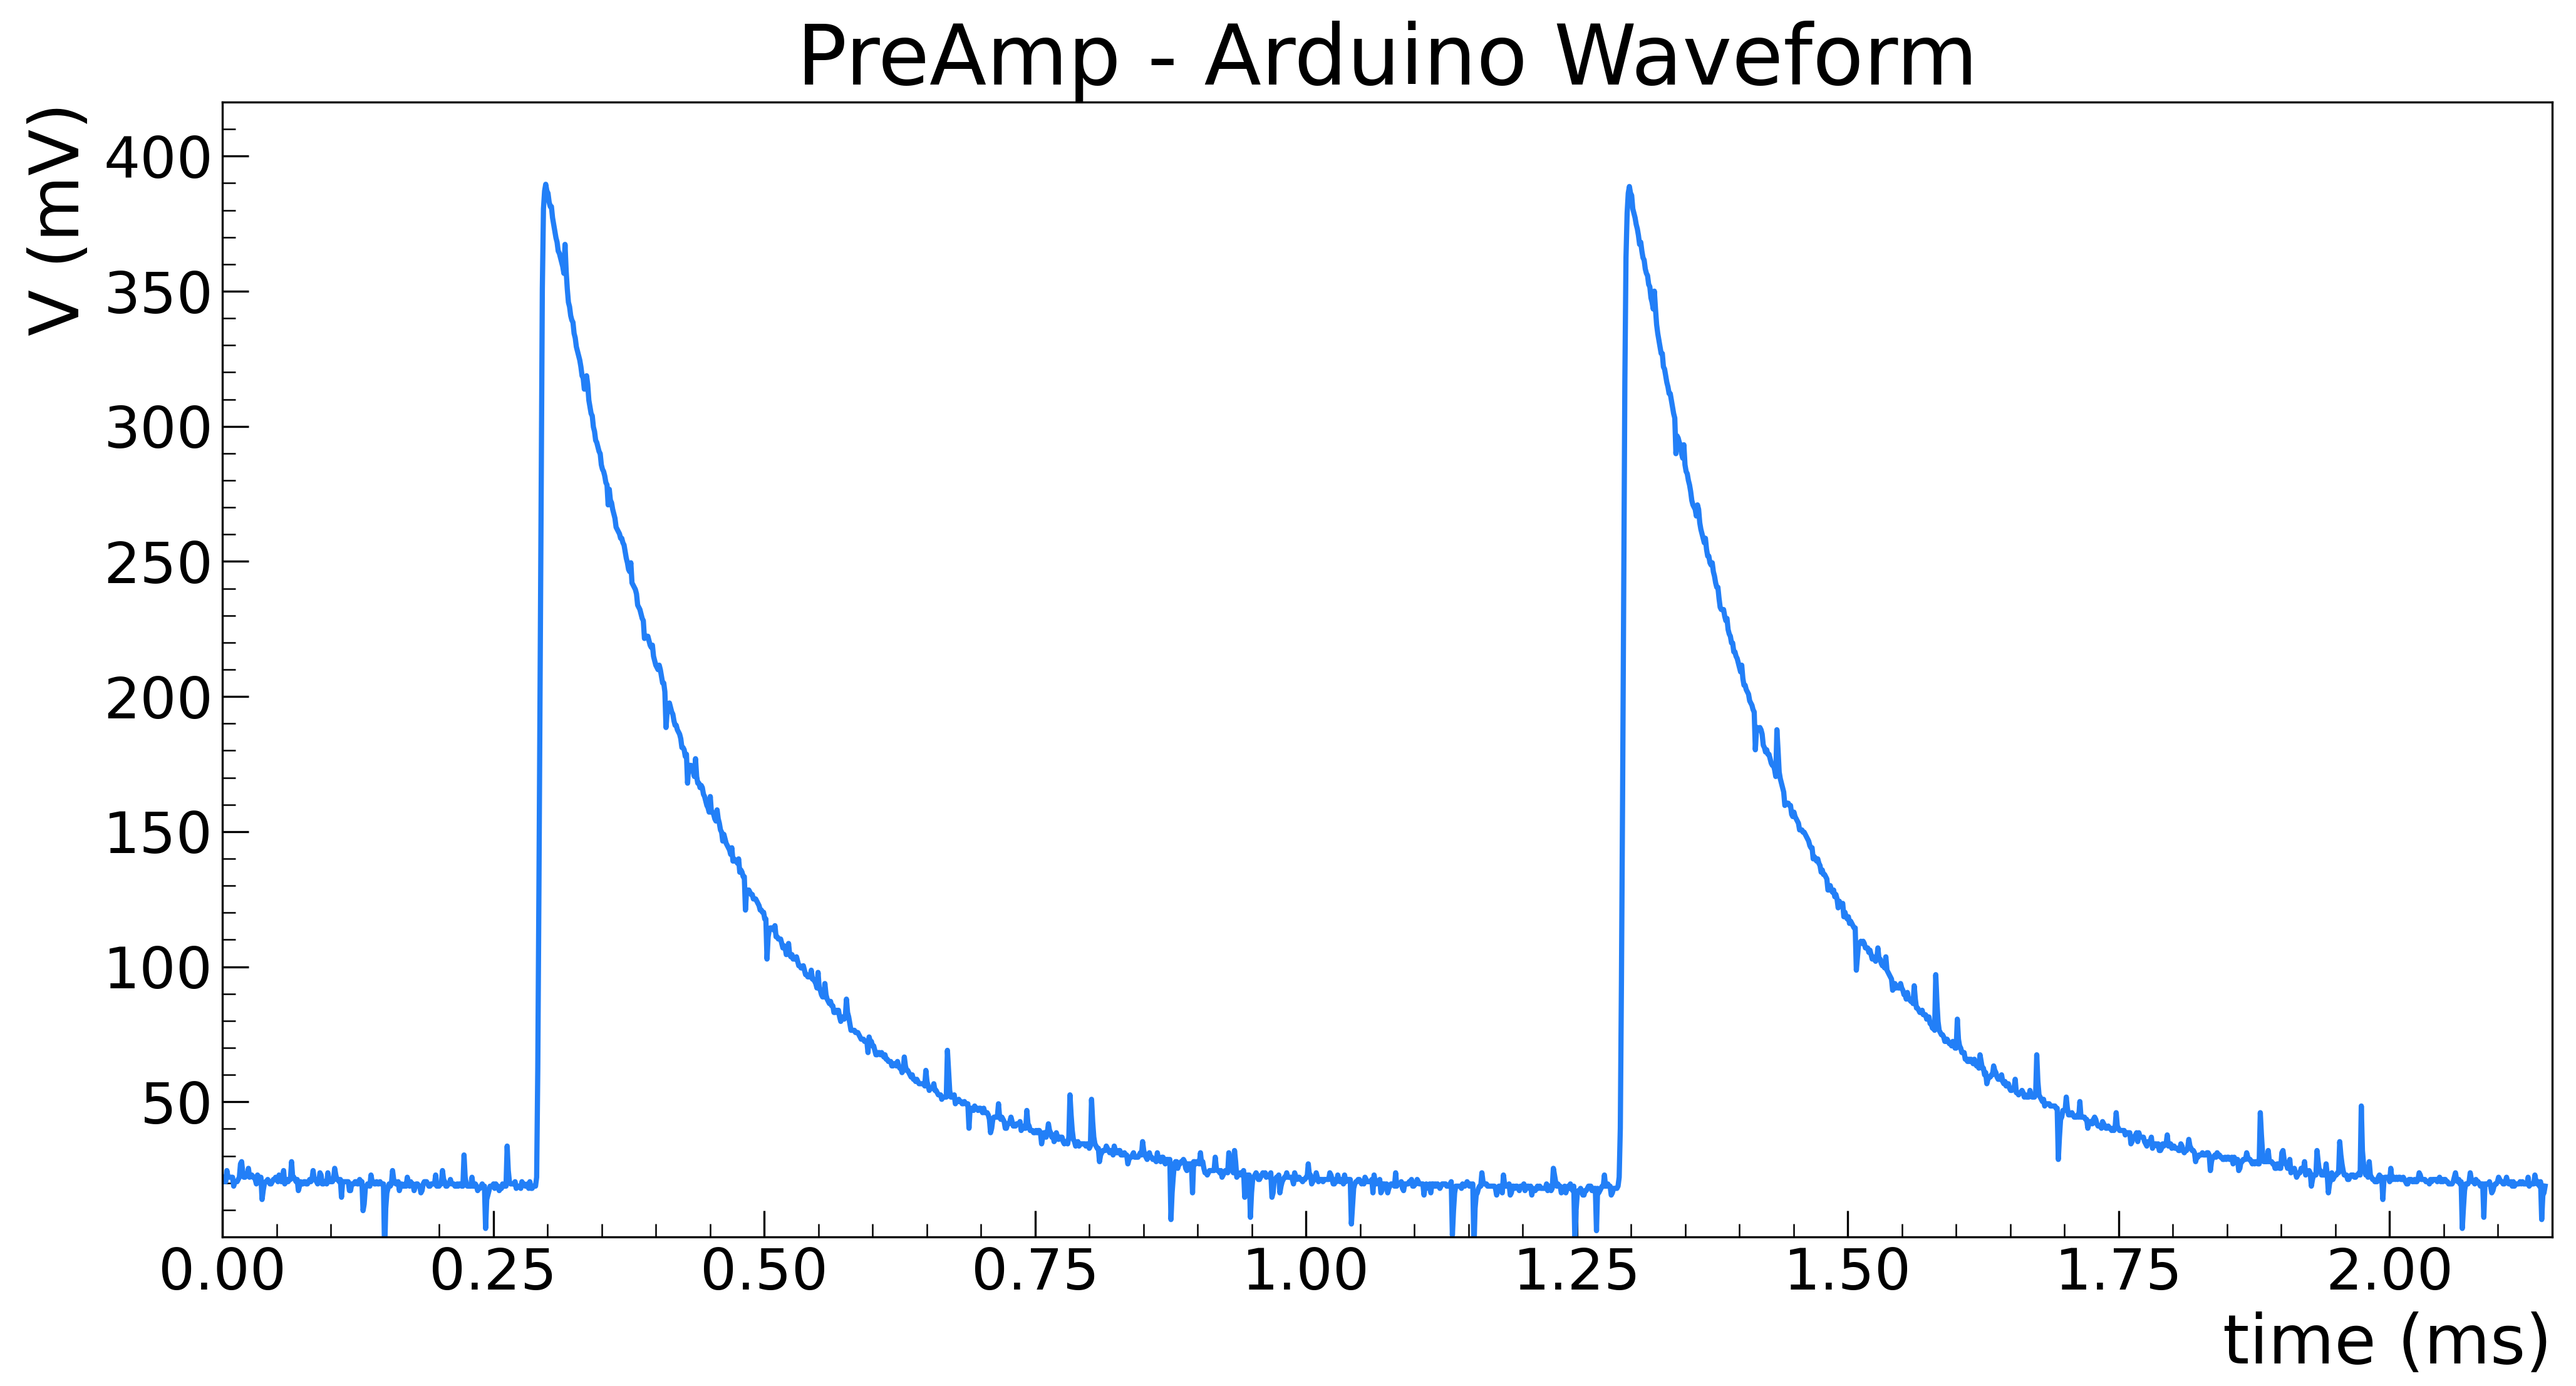
\includegraphics[width=0.5\textwidth]{../Plots/PreAmp/preamp_waveform.png}
 	\caption{\small Segnale in uscita dal preamplificatore.}
 	\label{i:preamp_waveform}
 \end{wrapfigure}

Osservando la \autoref{i:preamp_waveform}, si può inoltre notare chiaramente la salita lineare del segnale e la
decrescita esponenziale, come previsto in \autoref{e:preamp_vout}. Il valore massimo di tensione acquisito con la scheda
Arduino, inoltre, è in linea con le aspettative e con quanto misurato sperimentalmente con l'oscilloscopio. Ci si
concentra ora sulla stima del tempo caratteristico $\tau_{\text{pre}}$: si vuole inizialmente effettuare un fit
esponenziale del tipo $y = a + b\,\text{exp}(-x/\tau)$. Successivamente, sfruttando i parametri $a$ e $b$ per
normalizzare i dati, si vuole considerare il logaritmo delle tensioni normalizzate ed effettuare una regressione
lineare. Non è infatti possibile, per questioni analitiche, considerare semplicemente il logaritmo delle tensioni $V$ ed
aspettarsi un andamento lineare: si considera invece il logaritmo delle tensioni normalizzate $\tilde{V} = (V-a)/b$ e
l'errore su $\tilde{V}$ è dato per propagazione. In questo modo, quindi, i dati si distribuiscono secondo
$\log(\tilde{V})= -\frac{t}{\tau}$. 
 
\begin{figure}[H]
	\centering
	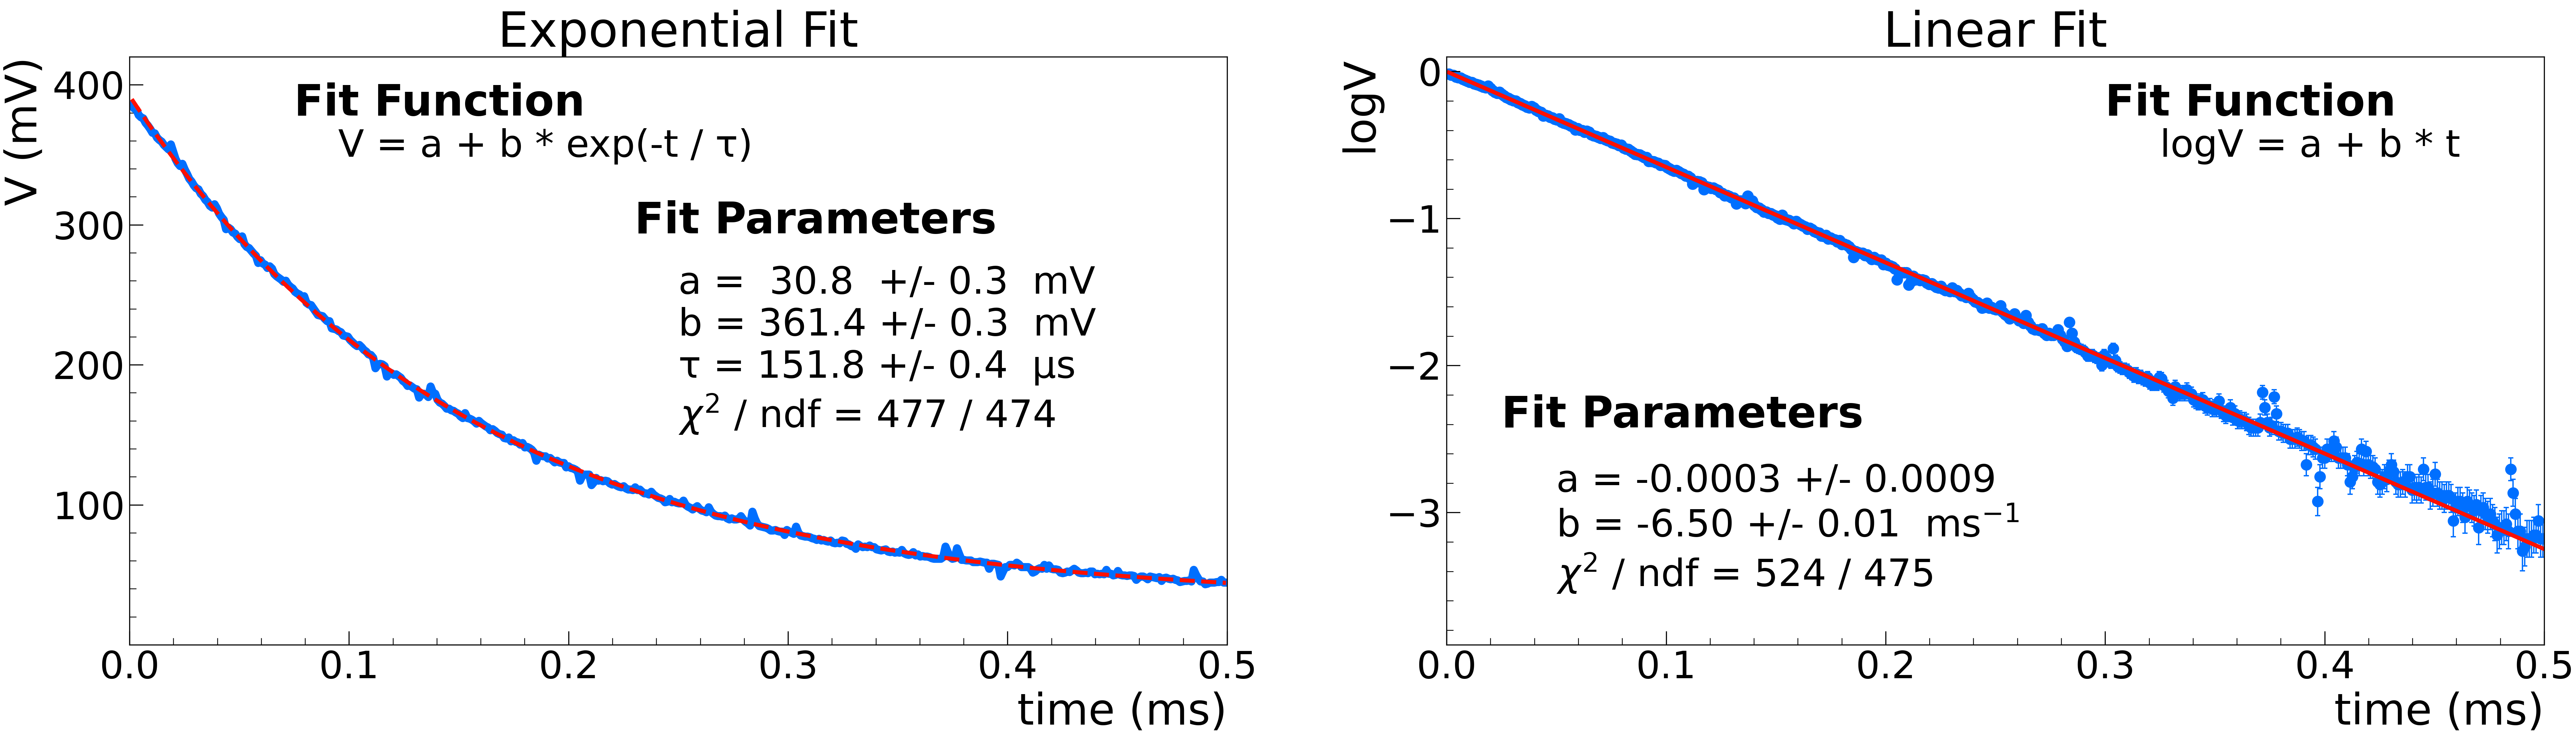
\includegraphics[width=\linewidth]{../Plots/PreAmp/preamp_arduino_fit2.png}
	\caption{\small A sinistra: fit esponenziale dello smorzamento del segnale in uscita. 
					A destra: fit lineare del logaritmo del segnale in uscita normalizzato.}
	\label{i:preamp_arduino_fit}
\end{figure}
 
Osservando rapidamente il grafico a sinistra, si nota come il segnale segua in modo ottimale la funzione esponenziale:
la stima del tempo caratteristico $\tau_{\text{pre}}^{\text{exp}}$, inoltre, risulta essere sufficientemente compatibile
con la stima teorica $\tau_{\text{pre}}^{\text{th}} = 161 \pm 6 \,\si{\us}$ ($\lambda = 1.5$). Come stima del tempo
caratteristico, in ogni caso, si preferisce quanto trovato dalla regressione lineare: tale metodo, infatti, è
complessivamente più robusto, più preciso e fornisce una stima migliore sugli errori dei parametri. Dal grafico a
destra, quindi, si nota chiaramente come computare il logaritmo delle tensioni $\tilde{V}$ porti a considerare più
"pesanti" (barre d'errore più piccole) i punti a monte della discesa esponenziale e a dare conseguentemente meno peso ai
punti di coda. Questi ultimi, eccessivamente prossimi allo zero, non vengono considerati dato che la propagazione
dell'errore su di essi porta ad un contributo decisamente troppo grande ed il fit non ne è praticamente influenzato. Il
$\chi^2$, inoltre risulta essere in soddisfacente accordo con il suo valore di aspettazione ($Z = 1.6$): le misure in
cima alla discesa si distribuiscono estremamente fedelmente attorno alla retta, compatibilmente con il loro errore,
mentre le misure verso la coda risultano discostarsi più sensibilmente dal fit. Si nota, infine, che rimuovendo dati
outlier scartando tutti i punti che distano più di $3\sigma$ dalla retta di regressione i risultati non vengono
sensibilmente influenzati: queste misure si trovano quasi esclusivamente sulla coda di destra e, avendo un errore
notevolmente maggiore rispetto ai punti situati in alto a sinistra, hanno poca influenza sulla retta del fit. Calcolando
ora il tempo caratteristico si trova $\tau_{\text{pre}}^{\text{lin}}= -1/b = 153.9 \pm 0.2 \,\si{\us}$: questo presenta
infine una compatibilità $\lambda = 1.2$ con  la stima teorica $\tau_{\text{pre}}^{\text{th}}$ ed è in linea con quanto
misurato sperimentalmente (\autoref{t:preamp_sper_th}).


%-------------------------------------------------------------------------------------------------------------------------------------------
%	THEBODE
%-------------------------------------------------------------------------------------------------------------------------------------------

\subsection{Analisi in Frequenza}\label{s:preamp_bode}

Si vuole ora studiare la risposta in frequenza del preamplificatore: si modificano le impostazioni del generatore in
modo da erogare un'onda sinusoidale di ampiezza $1\,\si{\volt}$ e frequenza $f_{\text{gen}}$ variabile da $10\,\si{\Hz}$
a $1\,\si{\MHz}$. Viene acquisita allora l'ampiezza del segnale sia in ingresso sia in uscita utilizzando
l'oscilloscopio e viene calcolata la funzione di trasferimento $H$, alla quale viene associata un'incertezza
$\sigma_{H}$ data da
\begin{align}\label{e:preamp_H_err}
	H&=\frac{V_{\text{out}}}{V_{\text{in}}} & 
	\sigma_{H}&= H \sqrt{	
						\left(	\frac{	\sigma_{\text{L}}\times V_{\text{in}}/\text{div}	}{	V_{\text{in}}	}	\right)^2	 + 
						\left(	\frac{	\sigma_{\text{L}}\times V_{\text{out}}/\text{div}	}{	V_{\text{out}}	}	\right)^2 }
\end{align}

dove $\sigma_{\text{L}}=0.04$ rappresenta l'incertezza di lettura associata all'oscilloscopio mentre i termini
$V_{\text{in}}/\text{div}$ e $V_{\text{out}}/\text{div}$ corrispondono al numero di Volt per divisione per il canale di
acquisizione rispettivamente del segnale in ingresso e del segnale in uscita. L'incertezza di guadagno associata
all'oscilloscopio non viene invece considerata in quanto, volendo rappresentare le misure acquisite sperimentalmente
attraverso un grafico di Bode, tale contributo viene scaricato interamente nell'intercetta delle interpolazioni volte a
caratterizzare l'andamento delle misure. L'errore sulle misure espresse in Decibel viene calcolato per propagazione. Si
assume infine trascurabile l'incertezza sulla frequenza dell'onda erogata dal generatore. Si faccia quindi riferimento a
quanto riportato in \autoref{s:preamp_th} per le aspettative teoriche della risposta in frequenza del circuito. Si
rappresenta ora in \autoref{i:preamp_thebode} il grafico di Bode delle misure acquisite assieme ai punti ottenuti
attraverso una simulazione Spice della risposta del circuito.

\begin{figure}[H]
	\centering
	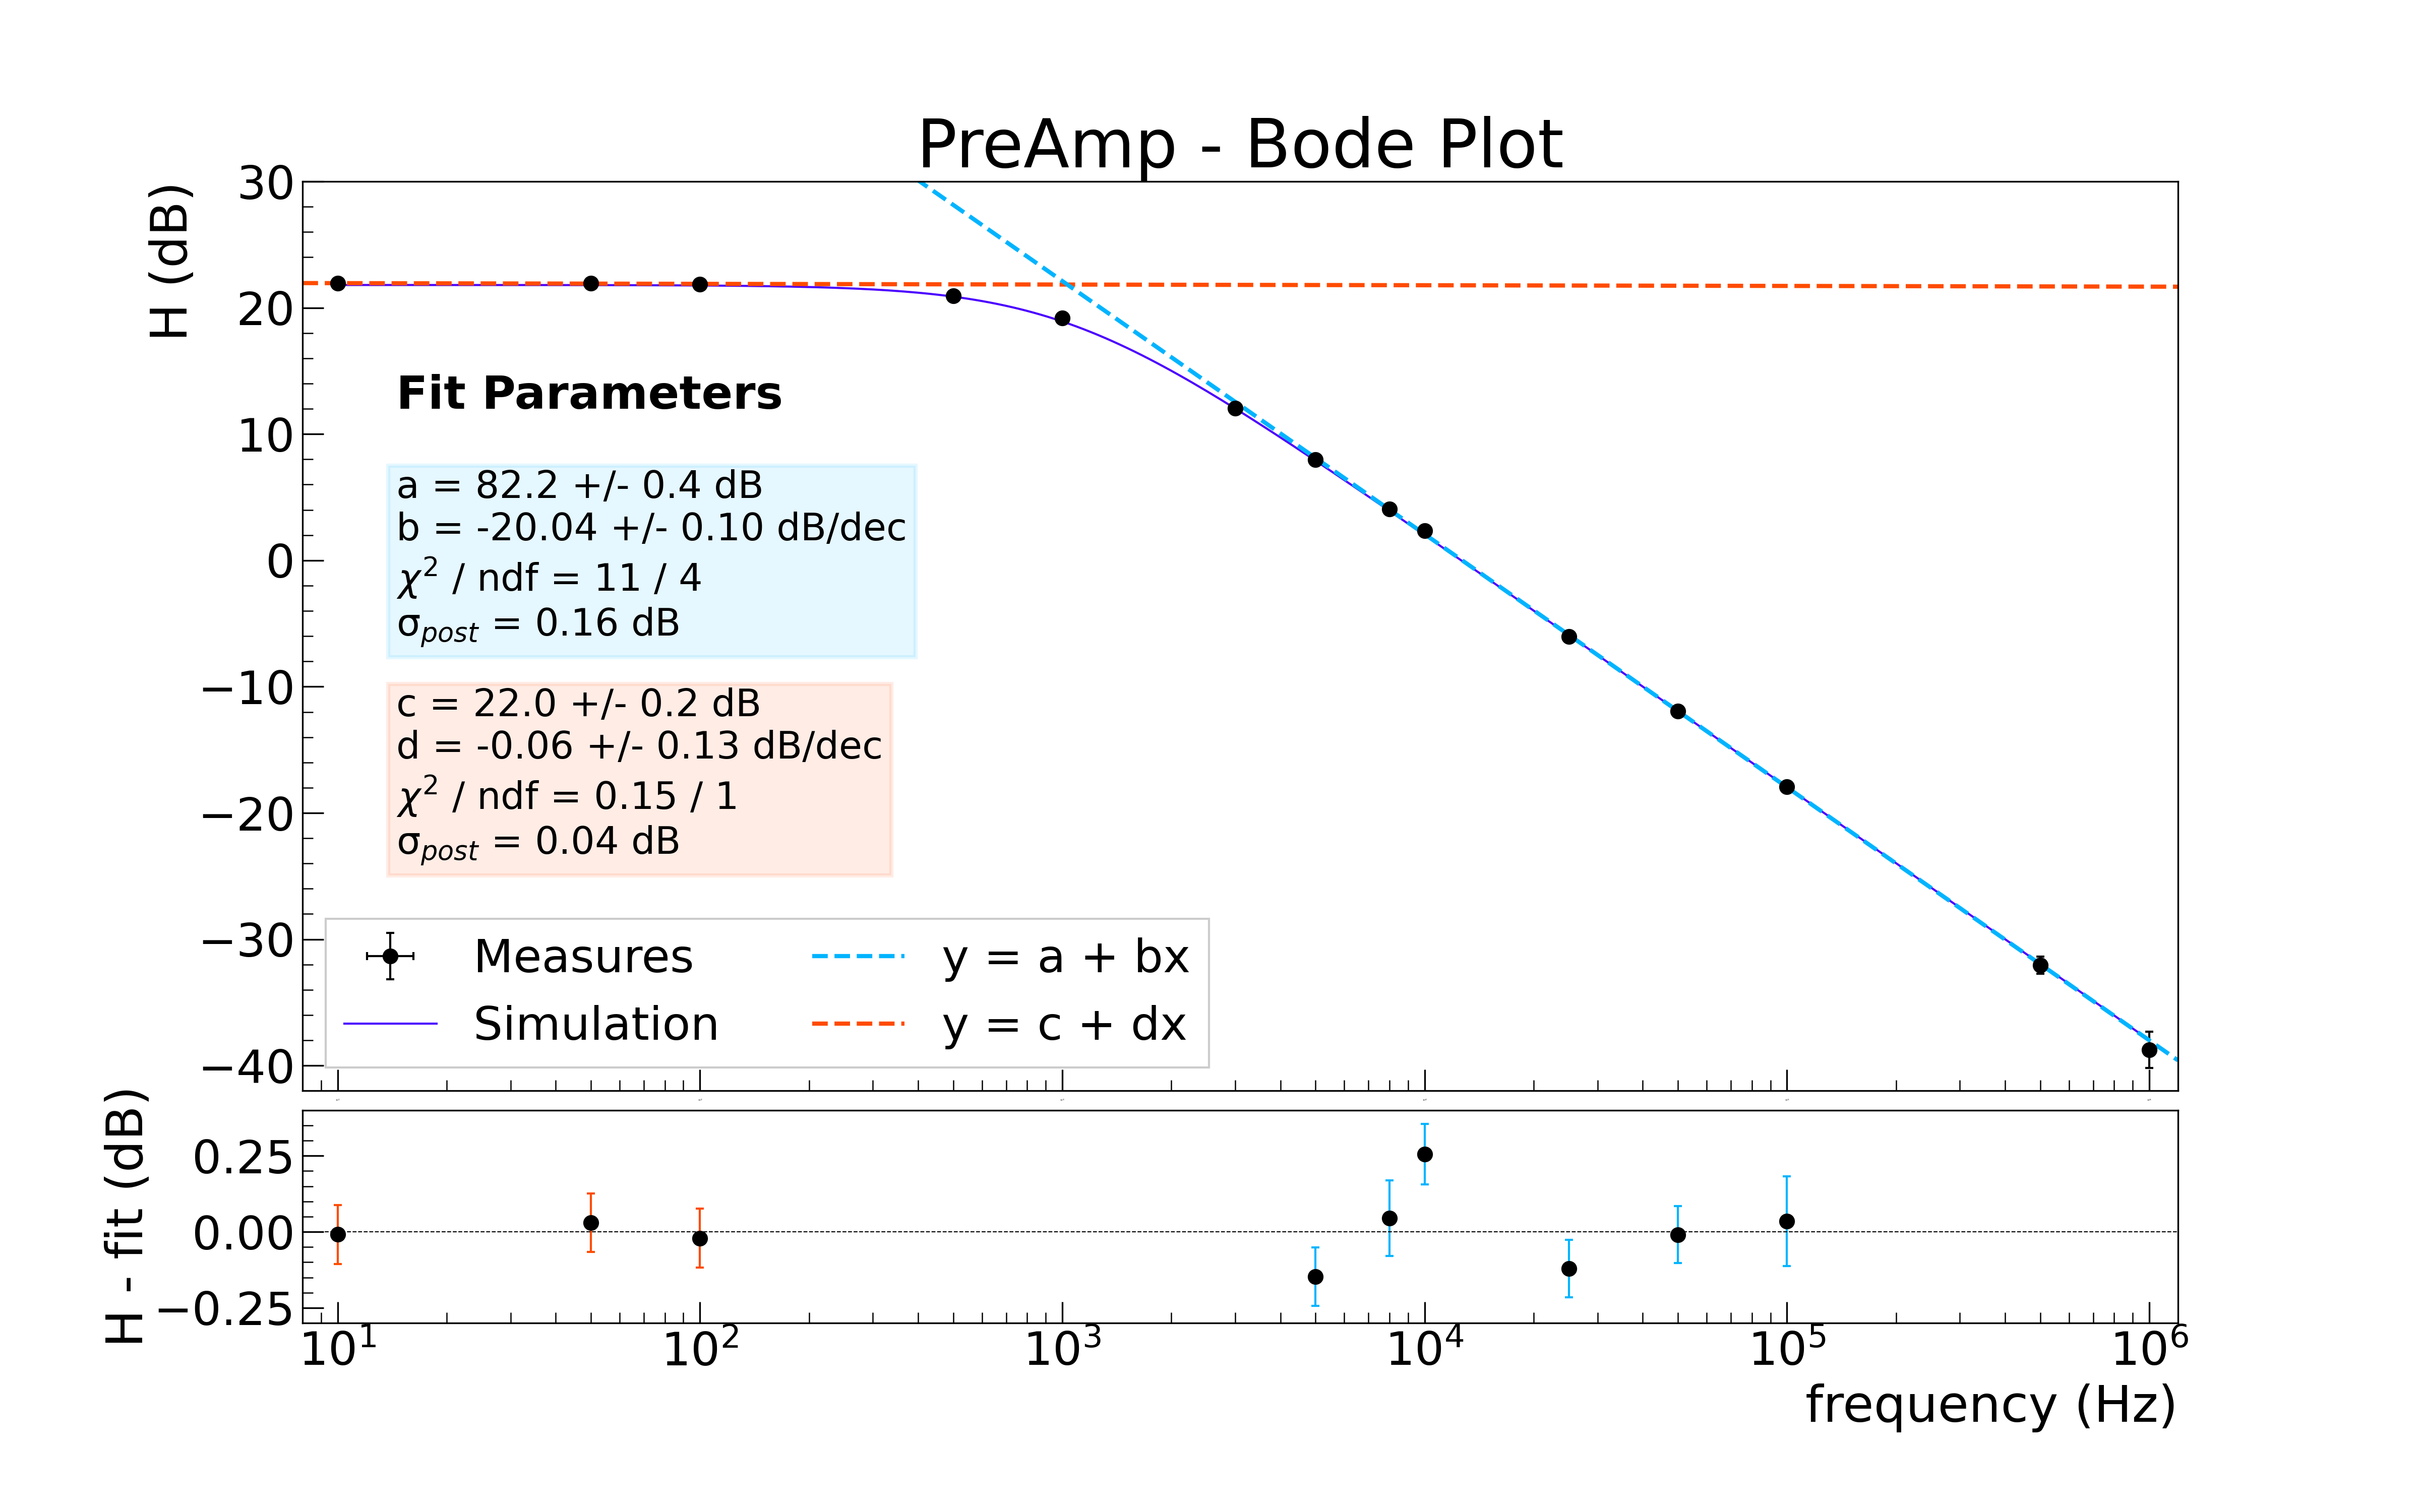
\includegraphics[width=0.9\linewidth]{../Plots/PreAmp/bode_plot.png}
	\caption{\small Grafico di Bode delle misure sperimentali e dei dati simulati.}
	\label{i:preamp_thebode}
\end{figure}

Confrontando inizialmente le misure sperimentali con la simulazione Spice, si nota un ottimo accordo in tutto lo spettro
di frequenze. Questo è chiaramente indice di una risposta in frequenza del circuito compatibile con le aspettative: il
comportamento del filtro, infatti, è evidentemente un passa basso. A basse frequenze, la funzione di trasferimento è
pressochè costante a $22\,\si{dB}$ (retta in \textit{arancione}), mentre per frequenze crescenti la funzione di
trasferimento decresce linearmente con coefficiente angolare conforme all'aspettativa dei $-20\,\si{dB/dec}$. L'ascissa
del punto di intersezione tra le due rette di regressione fornisce una stima della frequenza di taglio del circuito
$f_{\text{t}} = 1.03 \pm 0.03 \,\si{\kHz}$, compatibile in modo soddisfacente ($\lambda = 0.9$) con la frequenza di
taglio teorica esposta in \autoref{e:preamp_stime_th}. Si vuole sottolineare che nel computo dell'errore su
$f_{\text{t}}$ è stata presa in considerazione la covarianza tra parametri appartenenti allo stesso fit. Osservando
infine che la formula analitica frequenza di taglio $f_{\text{t}}$ riportata in \autoref{e:preamp_stime_th} contiene il
tempo caratteristico $\tau_{\text{pre}}$, si vuole valutare l'accordo tra la frequenza di taglio ottenuta dal grafico di
Bode e la frequenza di taglio teorica, utilizzando però $\tau_{\text{pre}}=\tau_{\text{pre}}^{\text{lin}}$ ricavato
nella sezione precedente. Si ottiene dunque una frequenza di taglio $f_{\text{t}}^{\text{lin}} = 1.0340 \pm 0.0013
\,\si{\kHz}$ ed è in eccellente compatibilità con quanto appena stimato ($\lambda = 0.13$). Da questo notevole accordo
si deduce l'assenza di possibili sistematicità di metodo, sia nella stima del tempo caratteristico attraverso il fit
lineare in \autoref{i:preamp_arduino_fit}, sia nella stima della frequenza di taglio analizzando il grafico di Bode. 


%-------------------------------------------------------------------------------------------------------------------------------------------
%	SHAPER
%-------------------------------------------------------------------------------------------------------------------------------------------

\section{Shaper CR-RC}\label{s:shaper} 

Riprendendo ora quanto esposto in \autoref{s:preamp_th}, si ottiene in uscita dal preamplificatore un segnale
dirattamente proporzionale alla carica in ingresso. Questo segnale è caratterizzato da una salita lineare fino al
raggiungimento del massimo di tensione (in modulo) $V_{\text{out}}^{\text{max}}=\frac{Q_{\text{c}}}{C_{\text{f}}}$ ed
uno smorzamento esponenziale di tempo caratteristico $\tau_{\text{pre}}$ di circa un centinaio di $\si{\us}$. Si nota
allora in \autoref{i:preamp_waveform} che un segnale di questo tipo impiega circa $1\,\si{\milli\second}$ per azzerarsi
completamente. Il secondo stadio della catena 

\begin{wrapfigure}{L}{0.5\textwidth}
	\centering
	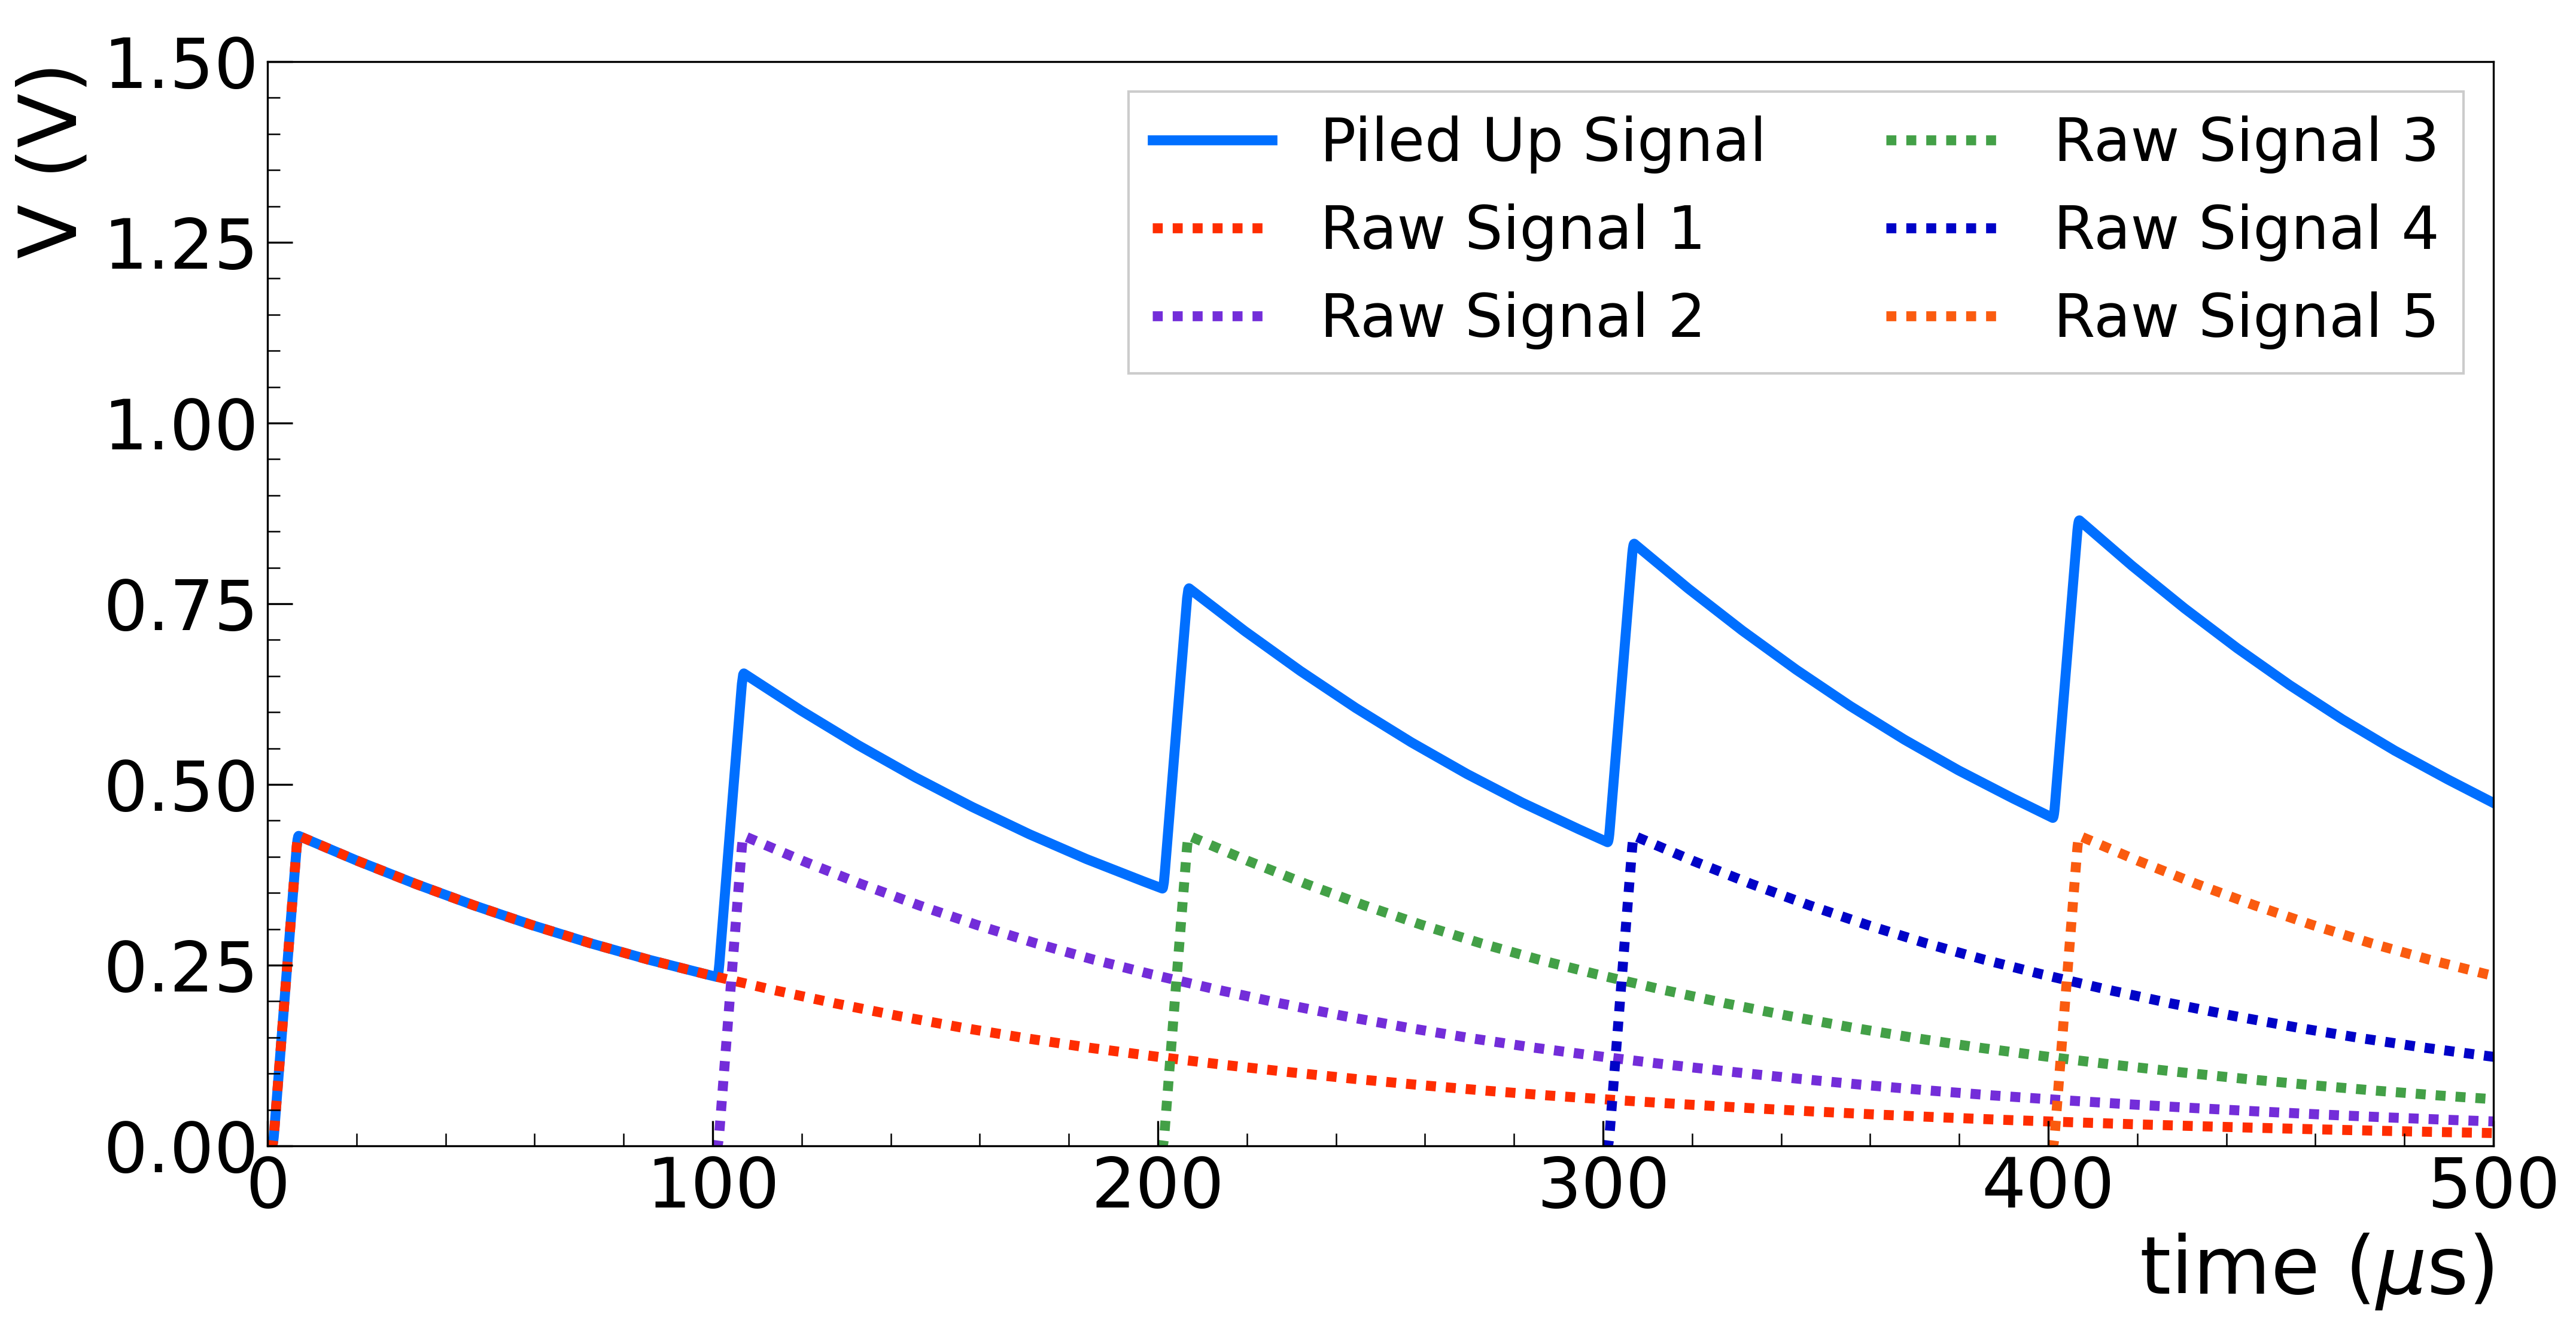
\includegraphics[width=0.5\textwidth]{../Plots/PreAmp/signal_pileup.png}
	\caption{\small Signal pile-up simulazione Spice.}
	\label{i:preamp_pileup}
\end{wrapfigure}

(\textit{shaper}) si utilizza per modificare la forma del segnale in uscita dal preamplificatore, rendendolo più simile
ad una curva gaussiana ed accorciandone la durata effettiva. Si è particolarmente interessati a diminuire il tempo di
discesa al fine di evitare un possibile \textit{signal pile up} nel caso di un'elevata frequenza di acquisizione. In
tale situazione, infatti, il segnale di un'acquisizione precedente si sovrapporrebbe (almeno parzialmente) a quello
dell'acquisizione successiva, rendendo estremamente più complicato estrarre le corrette informazioni dalle due
acquisizioni. In \autoref{i:preamp_pileup} è raffigurata una simulazione di questo fenomeno, impostando una frequenza
dell'impulso in ingresso pari a $10\,\si{\kilo\Hz}$. Infine, per quanto affermato in \autoref{s:preamp_th}, è importante
che lo shaper preservi l'informazione sulla carica in ingresso, in quanto questa risulta essere il modello utilizzando
nell'esperienza per simulare l'evento rivelato dal detector. Nelle sezioni successive si vuole ricavare analiticamente
il comportamento teorico dello shaper e, successivamente, verificarne l'accordo con la risposta sperimentale. In
particolare, si vuole verificare che il segnale in uscita sia proporzionale al segnale in ingresso e che la durata del
segnale in uscita sia ridotta rispetto allo smorzamento esponenziale della tensione dovuto al preamplificatore. Si vuole
sottolineare, infine, che inizialmente verrà studiato il comportamento dello shaper in condizioni di preamplificatore
\textit{ideale} mentre successivamente ci si concentrerà sul caso reale, il quale porta a delle leggere complicazioni.


%-------------------------------------------------------------------------------------------------------------------------------------------
%	CONFIGURAZIONE SPERIMENTALE IDEALE
%-------------------------------------------------------------------------------------------------------------------------------------------

\subsection{Configurazione Sperimentale Ideale}\label{s:shaper_config_ideale}

Si comincia assemblando sulla breadboard il secondo modulo rappresentato in \autoref{i:circuito} utilizzando le
resistenze e capacità riportate in \autoref{t:shaper_direct_measures}. Si evidenzia che per la prima fase di analisi
(preamplificatore ideale) non viene montata la resistenza $R_{\text{pz}}$. Per studiare il comportamento dello shaper in
coda ad 

\begin{wraptable}{L}{0.5\textwidth}
	\small
	\centering
	\begin{tabular}{x{1.8cm} x{2.5cm} x{2cm} } \toprule[0.5px]\toprule[0.1px]	
		\multicolumn{3}{c}{Misure Dirette - Shaper}\tn
		\midrule[0.1px]
		Label & Valore & F.S. \tn
		\addlinespace
		$R_{1}$ & $100.99 \pm 0.06\,\si{k\ohm}$ & $1000\,\si{k\ohm}$   \tn
		$R_{2}$ & $99.93  \pm 0.06\,\si{k\ohm}$ & $1000\,\si{k\ohm}$   \tn
		$C_{1}$ & $157    \pm 9 \,\si{n\farad}$ & $1000\,\si{p\farad}$ \tn
		$C_{2}$ & $159    \pm 9 \,\si{n\farad}$ & $1000\,\si{p\farad}$ \tn
		\bottomrule[0.5px]		
	\end{tabular}
	\caption{\small Misure dirette delle componenti circuitali.}
	\label{t:shaper_direct_measures}
\end{wraptable}	

un preamplificatore ideale è sufficiente fornire in ingresso (direttamente allo shaper) un segnale tale da avere una
salita (quasi) istantanea che mantenga la tensione al valore massimo per un tempo sufficientemente lungo. Un segnale di
questo tipo viene simulato facendo erogare al generatore di funzioni un'onda quadra a bassa frequenza ($100\,\si{\Hz}$)
di tensioni $V_{\text{low}} = 0\,\si{\volt}$ e $V_{\text{high}} = 1\,\si{\volt}$. Si rimanda infine a
\autoref{s:preamp_config} per l'alimentazione dell'operazionale e l'acquisizione del segnale mediante l'oscilloscopio.


%-------------------------------------------------------------------------------------------------------------------------------------------
%	TRATTAZIONE ANALITICA
%-------------------------------------------------------------------------------------------------------------------------------------------

\subsection{Trattazione Analitica}\label{s:shaper_th}

Si noti inizialmente (\autoref{i:circuito}) la presenza di un \textit{buffer} tra il modulo CR ed il modulo RC. Il \textit{buffer}, che non
altera il comportamento del circuito, permette di fattorizzare la funzione di trasferimento

\begin{wraptable}{R}{0.3\textwidth}
	\small
	\centering
	\begin{tabular}{x{3.5cm}} 
		\toprule[0.5px]
		\toprule[0.1px]	
		
		Shaping Time \tn

		\midrule[0.1px]
		
		\addlinespace

		$\tau_{\text{sh}1} = 15.86 \pm 0.91 \,\si{\us}$ \tn
		$\tau_{\text{sh}2} = 15.89 \pm 0.90 \,\si{\us}$ \tn

		\addlinespace

		$\langle\tau_{\text{sh}}\rangle = 15.9 \pm 0.6 \,\si{\us}$ \tn


		\bottomrule[0.5px]		
	\end{tabular}
	\caption{\small Stime del tempo caratteristico dello shaper.}
	\label{t:shaper_shaping_time}
\end{wraptable}	

 complessiva $H(s) = H_{\text{CR}} \, H_{\text{RC}}$, dove $H_{\text{CR}}$ e
$H_{\text{RC}}$ sono rispettivamente le funzioni di trasferimento di un circuito RC in configurazione passa alto e passa
basso. In questo modo, quindi, il calcolo della funzione di trasferimento si semplifica notevolmente. Inoltre, si vuole
assumere $R_1 \, C_1 \equiv \tau^{\text{sh}}_1 \approx \tau^{\text{sh}}_2 \equiv R_2 \, C_2$: questa approssimazione
risulta ragionevole osservando i valori riportati \autoref{t:shaper_shaping_time} e, di conseguenza, si considera la
media pesata dei due come tempo caratteristico dello shaper, detto \textit{shaping time}. L'effettiva validità di questa
approssimazione può essere verificata studiando il grafico di Bode della risposta in frequenza del circuito. La funzione
di trasferimento risulta allora essere

\begin{align}\label{e:shaper_H} 
	H(s) &= \frac{ 1 }{ \tau_{\text{sh} } }  \,  
	\frac{ s }{ \left( s + \frac{ 1 }{ \tau_{\text{sh} } } \right)^2}  
   	& 
   	&\text{con} \,\,\,\, \tau_{\text{sh}}= 15.9 \pm 0.6 \,\si{\us} 
   	\,\,\,\,\Longrightarrow\,\,\,\,
   	f_{\text{polo}}=\frac{1}{2\pi \tau_{\text{sh}}}= 10.0 \pm 0.4 \,\si{k\Hz}
\end{align}

Si noti quindi come la forma analitica di $H(s)$ presenti uno zero nell'origine ed un polo doppio legato allo
\textit{shaping time}. Il grafico di Bode della risposta in frequenza presenta allora una salita lineare con pendenza
$20\,\si{dB/dec}$ fino al raggiungimento della frequenza $f_{\text{polo}}$ relativa al polo doppio per poi decrescere
linearmente con pendenza $-20\,\si{dB/dec}$. Il filtro è dunque un passa banda, la cui banda passante (e di conseguenza
gli intervalli di integrazione e derivazione del segnale) è influenzata dallo \textit{shaping time}. Concentrando ora
l'attenzione sulla risposta dello shaper ad un segnale in ingresso ideale, ci si aspetta in uscita una tensione data da 
\begin{equation} 
	V_{\text{out}}(t)=\frac{V_{\text{in}}}{\tau^{ \text{sh} }} \, t \,
	e^{-\frac{t}{\tau^{ \text{sh} } }} 
\end{equation} 

che presenta un massimo $V_{\text{out}}^{\text{max}}= V_{\text{in}}/e$ direttamente proporzionale al segnale in
ingresso, che quindi contiene l'informazione sulla carica raccolta dal preamplificatore. Inoltre, tale massimo viene
assunto ad un tempo $t^{\text{max}} = \tau_{\text{sh}}$: lo \textit{shaping time}, quindi, determina approssimativamente
la durata del segnale in uscita dallo shaper. Si noti che $\tau_{\text{sh}}$ è un ordine di grandezza inferiore rispetto
al tempo caratteristico $\tau_{\text{pre}}$: da questo si deduce quindi che la durata del segnale viene notevolmente
ridotta grazie all'azione dello shaper, come anticipato in \autoref{s:shaper}. \\

Al fine di verificare il corretto funzionamento dell'apparato sperimentale, si riportano in \autoref{t:shaper_sper_th}
le misure sperimentali del massimo della tensione e dello \textit{shaping time} $\tau_{\text{sh}}$ acquisite con
l'oscilloscopio. 

\begin{wraptable}{R}{0.50\textwidth}
	\small
	\centering
	\begin{tabular}{x{1.8cm} x{1.8cm} x{1.7cm} x{1.7cm}} \toprule[0.5px]\toprule[0.1px]	

		\multicolumn{4}{c}{Controllo Apparato - Shaper} \tn

		\midrule[0.1px]

		$V_{\text{max}}^{\text{th}} \,(\si{\milli\volt})$ & $V_{\text{max}}^{\text{sper}} \,(\si{\milli\volt})$ &
		$\tau_{\text{sh}}^{\text{th}} \,(\si{\us})$ & $\tau_{\text{sh}}^{\text{sper}} \,(\si{\us})$ \tn

		\addlinespace

		$372 \pm 6$ & $342 \pm 6$ & $15.9 \pm 0.6$ & $16 \pm 3$ \tn

		\bottomrule[0.5px]		
	\end{tabular}
	\caption{\small Confronto tra stime teoriche e misure sperimentali.}
	\label{t:shaper_sper_th}
\end{wraptable}	

Confrontando la misura di $V_{\text{max}}^{\text{sper}}$ con l'aspettativa teorica emerge una sensibile discrepanza tra
le due: la prima, infatti, si discosta del $7.9\%$ rispetto alla seconda. Questa incongruenza si attribuisce
principalmente alle componenti circuitali ed alle sistematiche presenti nel circuito stesso, comprendendo quindi anche
la capacità parassita dovuta ai cavi ed alla breadboard. Tale valore massimo, tuttavia, viene assunto ad un tempo
$\tau_{\text{sh}}^{\text{sper}}$ perfettamente conforme allo \textit{shaping time}. 




%Avendo misurato con l'oscilloscopio il segnale in ingresso, ci si aspetta allora un segnale massimo in uscita
%$V_{\text{th}}^{\text{max}}= 0.372 \pm 0.006\,\si{\volt}$, mentre sperimentalmente si misura
%$V_{\text{sper}}^{\text{max}}= 0.342 \pm 0.006\,\si{\volt}$: quest'ultimo si discosta del $7.9\%$ rispetto al primo.
%Questa incongruenza tra aspettativa teorica e misura sperimentale si attribuisce principalmente alle componenti
%circuitali ed alle sistematiche presenti nel circuito stesso. Il valore massimo $V_{\text{sper}}^{\text{max}}$ viene
%invece assunto ad un tempo conforme allo \textit{shaping time}. In \autoref{i:shaper_ideal} viene mostrato il segnale
%in uscita, acquisito con la scheda Arduino, assieme alla simulazione Spice: si nota chiaramente come la tensione
%sperimentale sia inferiore alle aspettative, come già anticipato. Si fa notare, tuttavia, che il valore massimo dei
%dati acquisiti risulta essere $0.34 \pm 0.02 \,\si{\volt}$ e questo viene assunto ad un tempo $t \approx
%15.9\,\si{\us}$ perfettamente in linea con quanto misurato sperimentalmente.

%\begin{wrapfigure}{R}{0.5\textwidth} 
%	\centering 
%	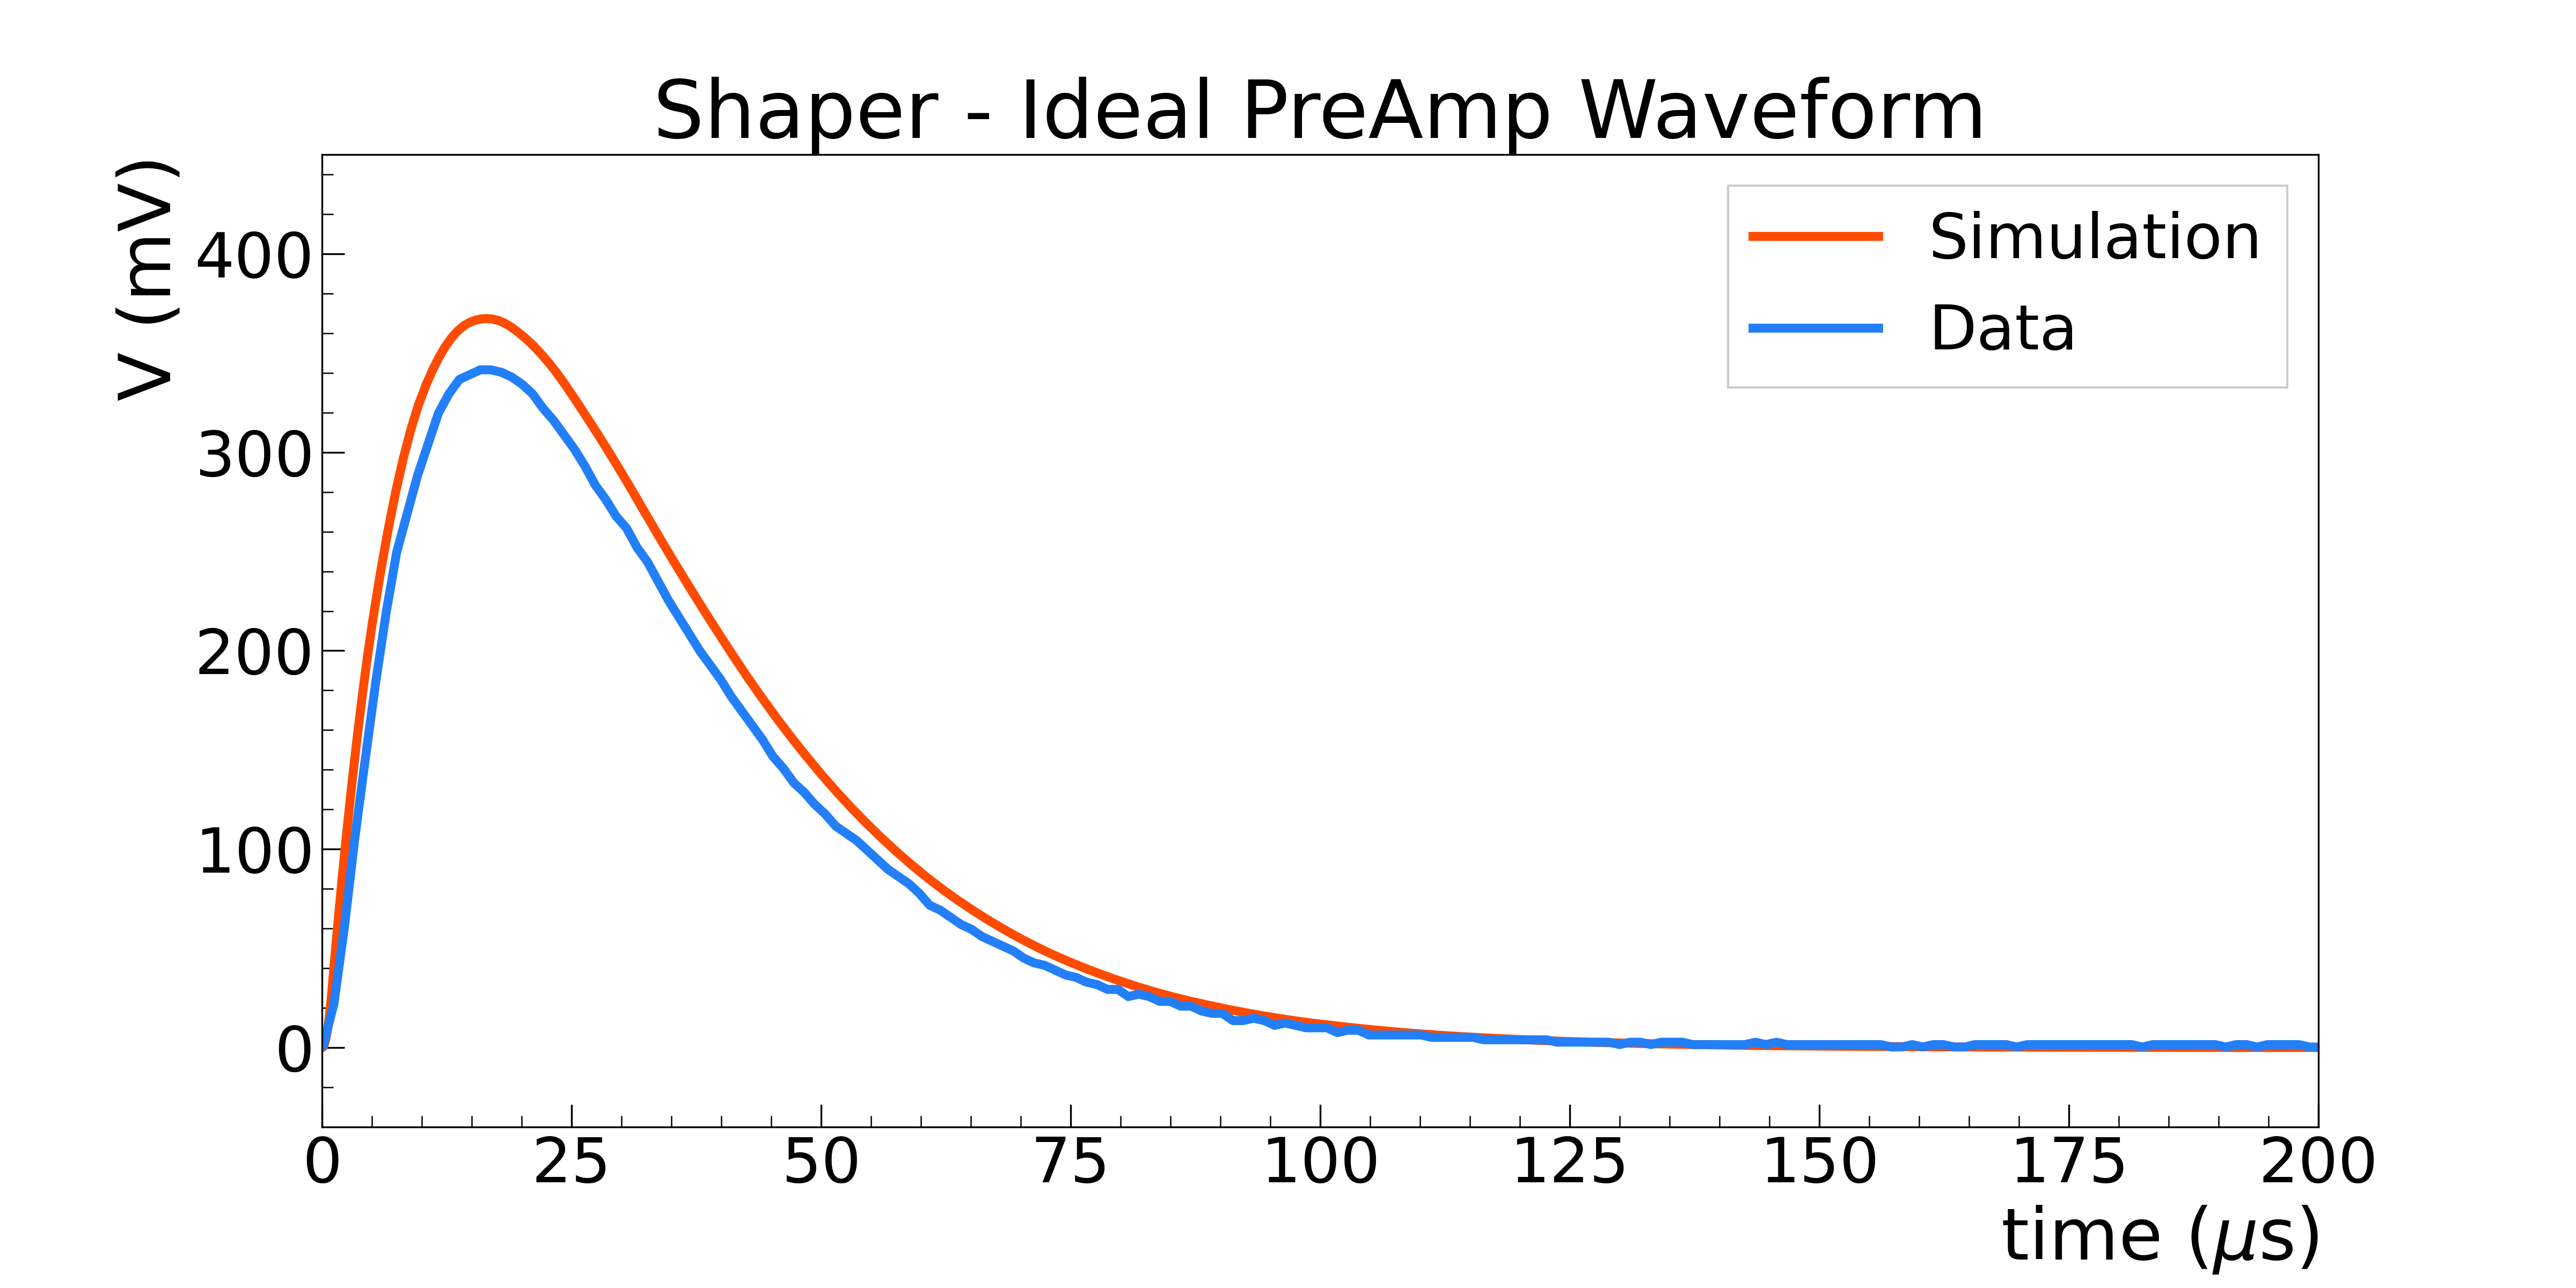
\includegraphics[width=0.5\textwidth]{../Plots/Shaper/shaper_ideal.png}
%   \caption{\small Segnale in uscita dallo shaper.} 
%   \label{i:shaper_ideal} 
%\end{wrapfigure}
%


%%-------------------------------------------------------------------------------------------------------------------------------------------
%%  THEBODE
%%-------------------------------------------------------------------------------------------------------------------------------------------
%
%\subsection{Analisi in Frequenza}\label{s:shaper_bode}
%
%Si vuole ora studiare la risposta in frequenza dello shaper: si imposta il generatore in modo da erogare un'onda
%sinusoidale di ampiezza $1\,\si{\volt}$ e frequenza $f_{\text{gen}}$ variabile da $50\,\si{\Hz}$ a $1\,\si{\MHz}$. Per
%quanto riportato in \autoref{e:preamp_H}, ci si aspetta un comportamento da filtro passa banda avente frequenza di
%massimo \begin{align}\label{e:shaper_ft_th} f_{\text{polo}}&=\frac{1}{2\pi \tau^{\text{sh}}}= 10.0 \pm 0.4 \,\si{k\Hz}
%& \text{con\,\,\,\,}\sigma_{f_{\text{polo}}}& =\frac{1}{2\pi}\frac{\sigma_{\tau^{\text{sh}}}}{\tau^{2}_{\text{sh}}}
%
%\end{align} \noindent  Si acquisisce quindi l'ampiezza del segnale sia in ingresso sia in uscita utilizzando
%l'oscilloscopio e viene calcolata la funzione di trasferimento $H$, alla quale viene associata un'incertezza
%$\sigma_{H}$ data da \autoref{e:preamp_H_err}. L'incertezza di guadagno associata all'oscilloscopio non viene invece
%considerata in quanto, dovendo successivamente prendere il logaritmo $\text{log}_{10}H$ della funzione di
%trasferimento, tale contributo viene scaricato interamente nell'intercetta delle interpolazioni volte a caratterizzare
%l'andamento delle misure. Si assume infine trascurabile l'incertezza sulla frequenza dell'onda erogata dal generatore.
%Si rappresenta allora in \autoref{i:shaper_thebode} il grafico di Bode delle misure acquisite assieme ai punti ottenuti
%attraverso una simulazione Spice della risposta del circuito (pagina seguente). Confrontando inizialmente le misure
%sperimentali con la simulazione Spice si nota un ottimo accordo a basse frequenze e nella zona di \textit{mid band},
%mentre per alte frequenze (attorno al MHz) si osserva un sensibile disaccordo tra misure sperimentali e simulazione
%Spice: la causa di questa anomalia si crede essere dovuta alla GBW dell'operazionale, la quale non è stata presa in
%considerazione nel simulare la risposta del circuito.\footnote{La \textit{Gain BandWidth} dell'amplificatore
%operazionale, anche detta \textit{frequenza a guadagno unitario}, determina il massimo guadagno ottenibile ad una data
%frequenza.} In ogni caso, il filtro si comporta come da aspettative: la funzione di trasferimento presenta una crescita
%lineare a basse frequenze (zona di derivazione) con pendenza $19.3 \pm 0.2 \,\text{dB/dec}$ ed una \newpage
%\begin{figure}[H] \centering 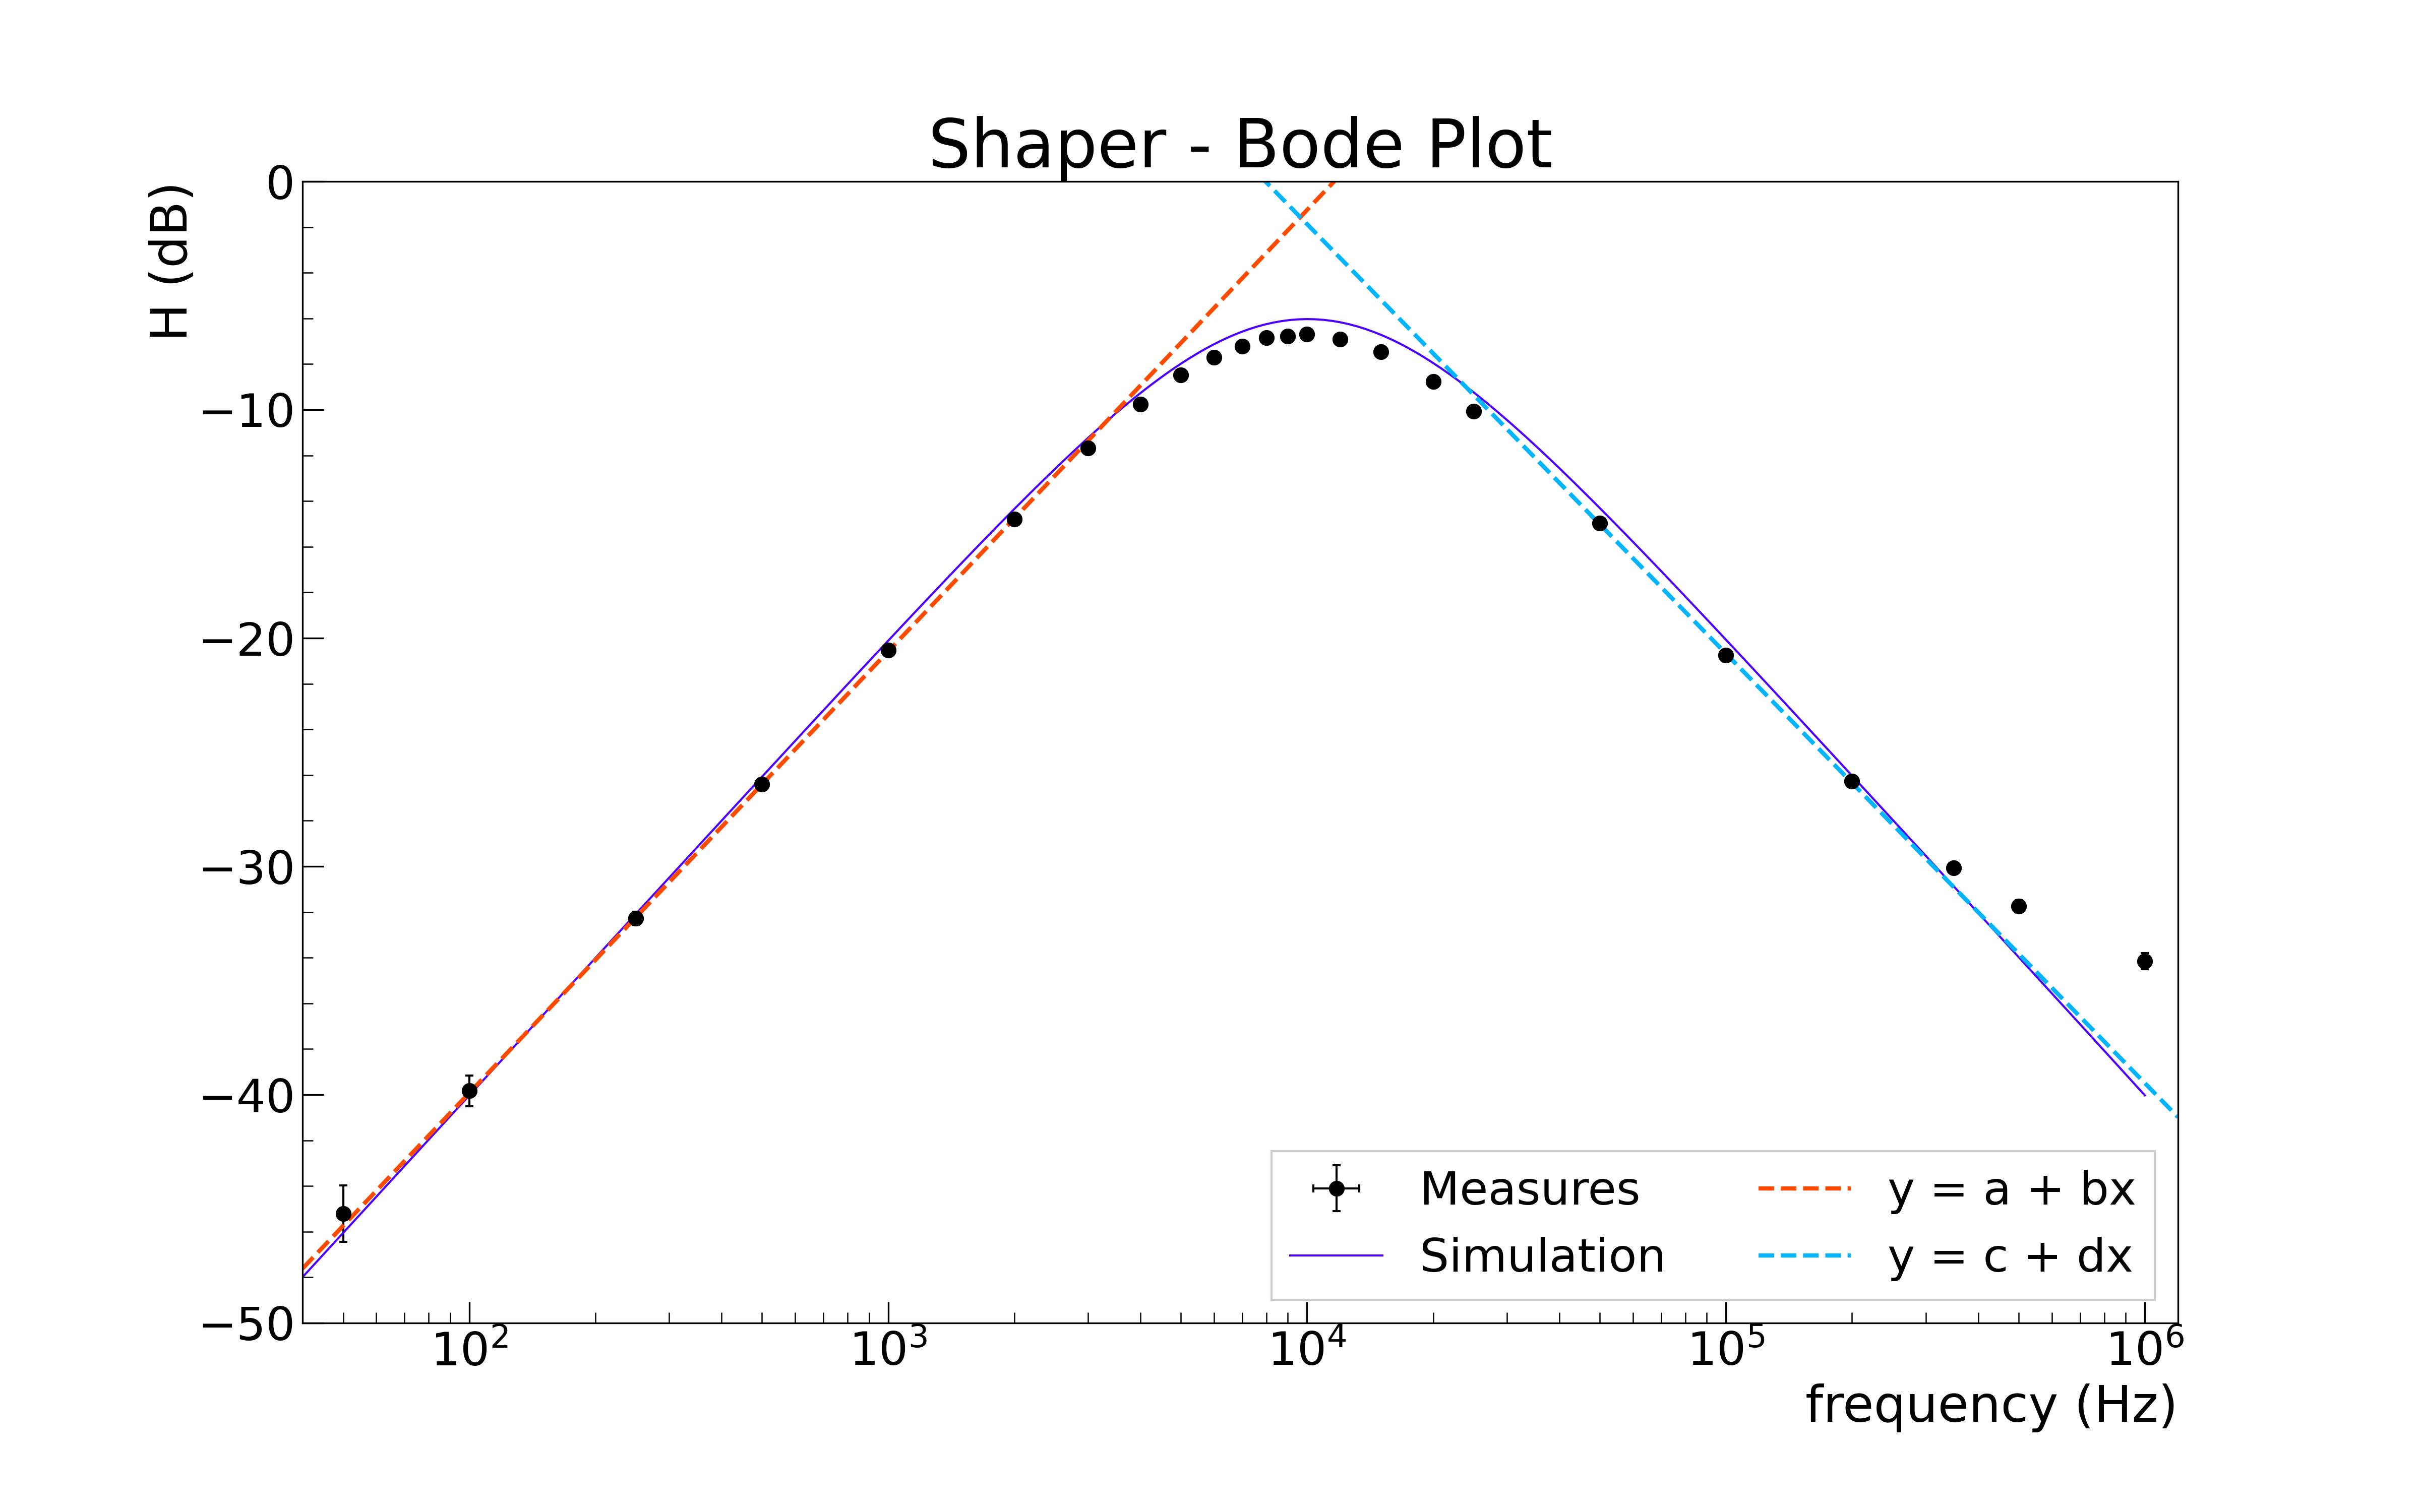
\includegraphics[width=0.9\linewidth]{../Plots/Shaper/bode_plot.png} \caption{\small
%Grafico di Bode delle misure sperimentali e dei dati simulati.} \label{i:shaper_thebode} \end{figure} \noindent
%decrescita lineare ad alte frequenze (zona di integrazione) con pendenza $-18.8 \pm 0.3 \,\text{dB/dec}$. L'ascissa del
%punto di intersezione delle due rette di regressione fornisce una stima della frequenza relativo al polo
%$f_{\text{polo}} = 9.6 \pm 0.2 \,\si{k\Hz}$, in ottima compatibilità con la frequenza del polo teorica esposta in
%\autoref{e:shaper_ft_th} ($\lambda = 0.8$). Partendo dalla stima ottenuta per $f_{\text{polo}}$, si ricerca il valore
%massimo della funzione di trasferimento: sottraendo infine $3\,\text{dB}$ a tale massimo e cercando le ascisse di
%intersezione con le due rette di regressione si riesce a determinare la larghezza di banda $\Delta f$ del filtro. Si
%ottiene quindi la \textit{mid band} dello shaper, delimitata da \begin{align}\label{e:shaper_bw} f_{\text{low}} &= 3.7
%\pm 0.4 \,\si{k\Hz} & f_{\text{high}} &= 26.1 \pm 0.8\,\si{k\Hz} \end{align} \noindent Si vuole infine sottolineare che
%l'ottimo accordo della frequenza $f_{\text{polo}}$ con l'aspettativa teorica (in cui compare la media pesata
%$\tau^{\text{sh}}$) supporta ulteriormente la validità dell'approssimazione $\tau^{\text{sh}}_1 \approx
%\tau^{\text{sh}}_2$.
%
%%-------------------------------------------------------------------------------------------------------------------------------------------
%%  SHAPER + PREAMP
%%-------------------------------------------------------------------------------------------------------------------------------------------
%
%\subsection{Shaper con Preamplificatore in ingresso}\label{s:shaper_preamp}
%
%In questa sezione si vuole studiare il comportamento dello shaper con in ingresso il segnale elaborato dal
%preamplificatore. Il generatore di funzioni viene configurato nuovamente come in \autoref{s:preamp_config}: impulso
%quadrato di frequenza $f_{\text{gen}} = 1 \,\si{k\Hz}$, tensione di riferimento $V_{\text{high}} = 0 \,\si{\volt}$,
%ampiezza \textit{negativa} $V_{\text{low}} = -1 \,\si{\volt}$ e durata $T = 5 \,\si{\us}$. In questa configurazione, il
%segnale in ingresso allo shaper corrisponde a quello rappresentato in \autoref{i:preamp_waveform}: la salita è ora
%lineare, non più "istantanea", ed il segnale è smorzato esponenzialmente, non più costante al valore massimo. Questa
%deviazione dall'idealità del segnale in ingresso allo shaper porta a rilevanti deformazioni del segnale in uscita:
%osservando il grafico a sinistra in \autoref{i:shaper_waveforms} si nota chiaramente il fenomeno di
%\textit{undershoot}. Il segnale, infatti, dopo aver raggiunto il massimo scende sotto allo zero (\textit{baseline}) per
%poi tendere ad esso abbastanza lentamente (nel caso ideale dopo $200\,\si{\us}$ il segnale si è già azzerato, in questo
%caso invece è necessario attendere circa $600\,\si{\us}$). La risoluzione di questo problema consiste nel porre una
%resistenza adeguata in parallelo alla capacità $C_{1}$: scegliendo questa tale che $R_{\text{pz}} =
%\frac{\tau^{\text{pre}}}{C_{1}}$, si trova $R_{\text{pz}} \gg R_{1}$ e di conseguenza la funzione di trasferimento
%\begin{align} H(s) &= \frac{s + \frac{ 1 }{ \tau^{ \text{pz} } }
%           }
%           {
%           s + \frac{ 1 }{ \tau^{ \parallel } }
%           } 
%       \approx
%       \frac{
%           s + \frac{ 1 }{ \tau^{ \text{pz} } }
%           }
%           {
%           s + \frac{ 1 }{ \tau^{ \text{1} } }
%           } &
%   &\text{con} \,\,\,\,    
%   \begin{cases} \tau^{ \text{pz} } = C_{ 1 }\, R_{ \text{pz} }  \\
%       \tau^{ \parallel } = C_{ 1 }\left(\frac{1}{R_{1}}+\frac{1}{R_{\text{pz}}}\right)^{-1}\\
%   \end{cases} \end{align} \noindent risulta, in buona approssimazione, avere lo stesso polo del modulo CR dello
%shaper. Di conseguenza, la funzione di trasferimento dello shaper con aggiunta la resistenza $R_{\text{pz}}$ continua
%ad avere un polo doppio in $f_{\text{polo}}$ e questo non ne altera le proprietà caratteristiche. La correzione
%apportata per eliminare l'effetto ti \textit{undershoot} prende il nome di compensazione \textit{pole zero}. In
%laboratorio, quindi, viene montata una resistenza $R_{\text{pz}} = 1.013 \pm 0.007 \, \si{\mega\ohm}$ ($\text{F.S.}
%10\,\si{\mega\ohm}$) molto simile a quella necessaria per compensare l'effetto di \textit{undershoot}
%($R_{\text{pz}}^{\text{th}} = 1.03 \pm 0.07 \, \si{\mega\ohm}$): osservando il grafico a destra in
%\autoref{i:shaper_waveforms} si nota quindi come l'effetto sia del tutto scomparso. Il segnale ora, infatti, dopo aver
%assunto il valore massimo decresce senza scendere sotto la \textit{baseline}. Inoltre, il segnale si azzera
%completamente dopo circa $200\,\si{\us}$, come nel caso ideale trattato in precedenza. \begin{figure}[H] \centering
%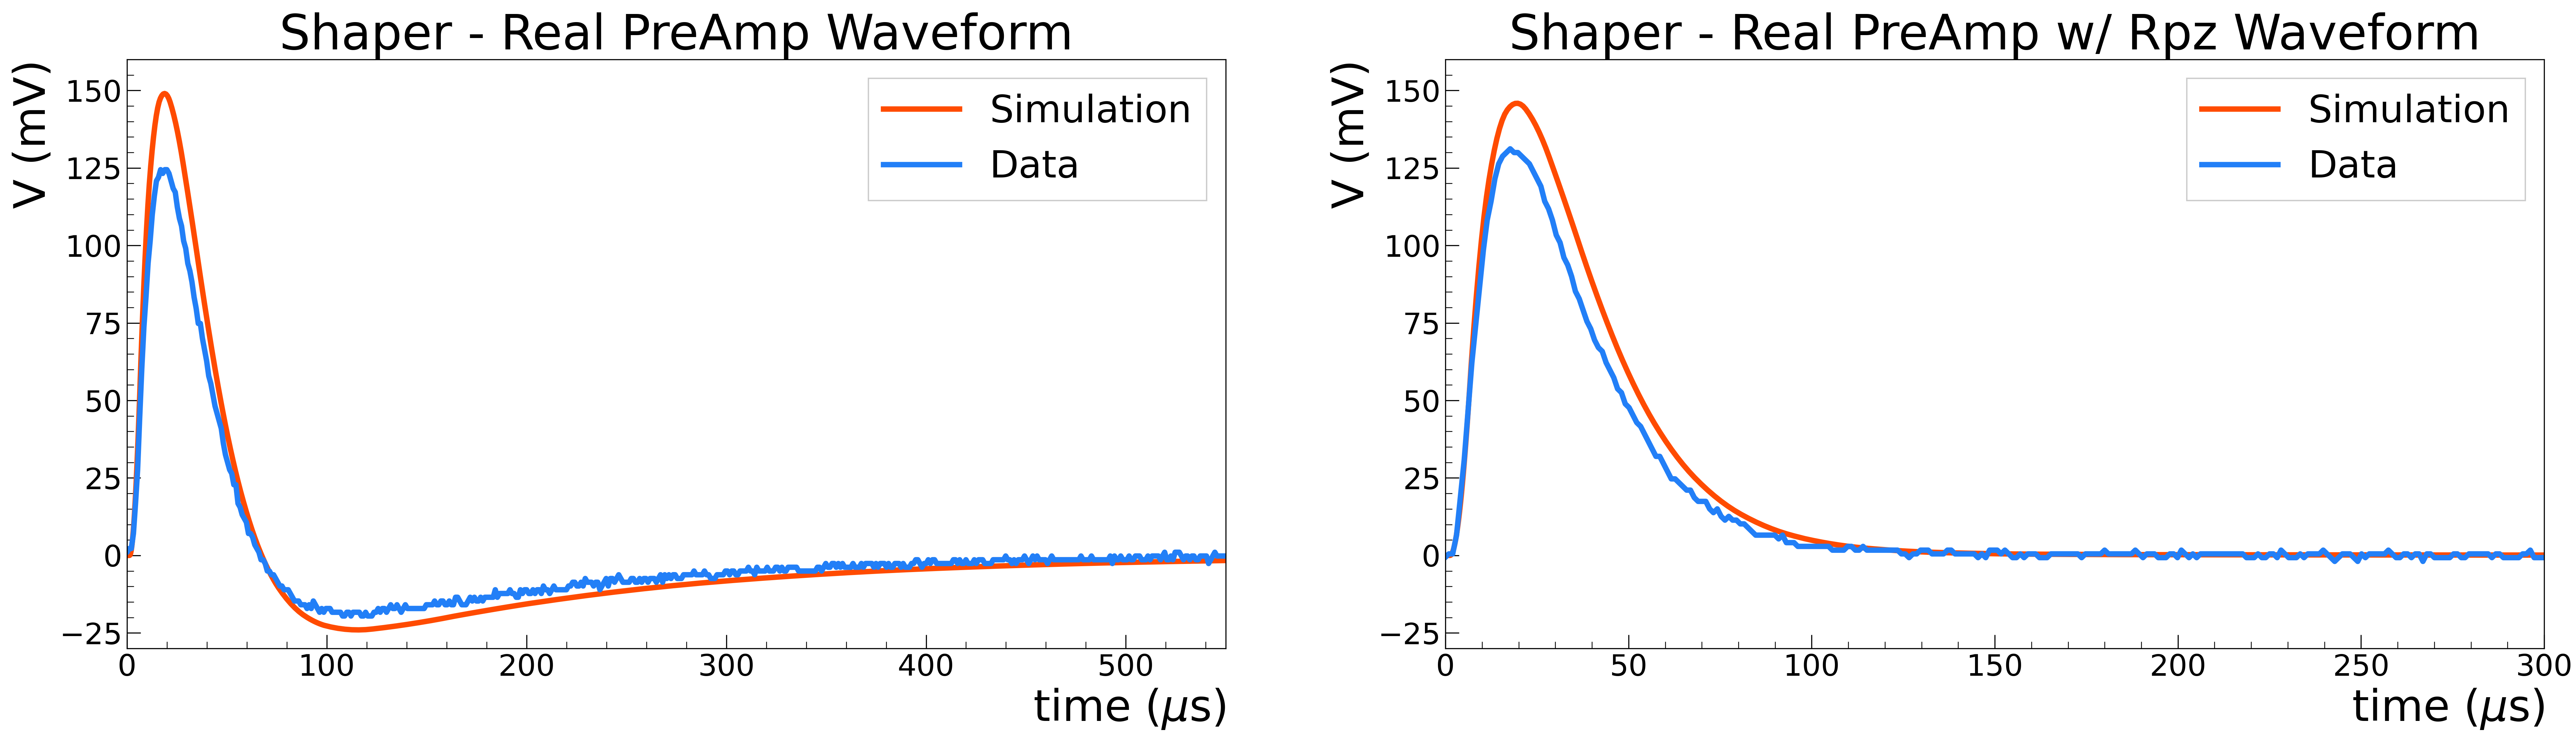
\includegraphics[width=\linewidth]{../Plots/Shaper/shaper_preamp_waveforms.png} \caption{\small A sinistra: segnale in
%uscita dallo shaper senza resistenza di compensazione. A destra: segnale in uscita dallo shaper con resistenza di
%compensazione.} \label{i:shaper_waveforms} \end{figure} \noindent Si vuole ora confrontare le misure sperimentali
%acquisite con l'oscilloscopio ed i dati acquisiti con la scheda Arduino. In \autoref{t:shaper_vout} si riportano quindi
%le misure del massimo della tensione $V_{\text{max}}$, il tempo in cui tale massimo viene assunto $t_{\text{max}}$ e,
%eventualmente, la tensione di \textit{undershoot} $V_{\text{undershoot}}$. 
%
%\begin{table}[H] \small \centering \begin{tabular}{x{2.2cm} x{2.2cm} | x{2.2cm} x{2.2cm} | x{2.2cm} x{2.2cm}}
%   \toprule[0.5px]\toprule[0.1px]   
%       \multicolumn{6}{c}{Shaper - Segnale in uscita \textit{senza} $R_{\text{pz}}$}\tn \midrule[0.1px]
%
%       \multicolumn{2}{c}{$V_{\text{max}} \,(\si{\milli\volt}) $} & \multicolumn{2}{c}{$t_{\text{max}} \,(\si{\us})$} & 
%       \multicolumn{2}{c}{$V_{\text{undershoot}} \,(\si{\milli\volt})$} \tn
%       Osc. & Arduino & Osc. & Arduino & Osc. & Arduino \tn
%
%       %\addlinespace
%
%       $ 123 \pm 2 $&$ 124 \pm 19 $&$ 17 \pm 1 $&$ \sim 16.8 $&$ -19.7 \pm 1.1 $&$ -20 \pm  17 $\tn
%
%       \midrule[0.1px]
%       \multicolumn{6}{c}{Shaper - Segnale in uscita \textit{con} $R_{\text{pz}}$}\tn
%       \midrule[0.1px]
%
%       \multicolumn{2}{c}{$V_{\text{max}} \,(\si{\milli\volt}) $} & \multicolumn{2}{c}{$t_{\text{max}} \,(\si{\us})$} & 
%       \multicolumn{2}{c}{$V_{\text{undershoot}} \,(\si{\milli\volt})$} \tn
%       Osc. & Arduino & Osc. & Arduino & Osc. & Arduino \tn
%
%       %\addlinespace
%
%       $ 129 \pm 2 $&$ 131 \pm 19 $&$ 17 \pm 1 $&$ \sim 17.7 $& \xmark & \xmark \tn
%
%       \bottomrule[0.5px]      
%   \end{tabular} \caption{\small Confronto del segnale in uscita tra le due configurazioni dello shaper.}
%   \label{t:shaper_vout} \end{table}    
%\noindent Si noti allora come tutte le misure acquisite con l'oscilloscopio e con Arduino sono tra loro consistenti.
%Inoltre, risulta evidente una notevole differenza di precisione tra le due tipologie di acquisizione: per quanto
%riguarda le misure di tensione l'oscilloscopio si trova essere circa un ordine di grandezza più preciso. L'errore
%relativo sulla misura del massimo $V_{\text{max}}$, infatti, risulta essere per l'acquisizione con Arduino di circa il
%$15\%$, mentre per l'acquisizione con l'oscilloscopio si trova circa $1.6\%$. %potrebbe essere perchè non sto
%sfruttando tutti i 4000 bit di arduino!! è fatto apposta per essere più preciso quando %le tensioni sono grandi?
%Osservando l'accordo tra misure acquisite con Arduino e le simulazioni Spice, invece, si nota una lieve discrepanza.
%Questo era già stato osservato in \autoref{i:shaper_ideal}: il segnale misurato sia con la scheda Arduino sia con
%l'oscilloscopio risulta essere sempre leggermente minore delle aspettative. Si ritiene, tuttavia, più rilevante
%l'elevato accordo tra metodologie di acquisizione differenti, piuttosto che la lieve discrepanza con simulazioni. Come
%si è già fatto notare, infatti, questa deviazione dalle aspettative teoriche viene associata a delle sistematiche
%inerenti alle componenti circuitali ed all'assemblaggio del circuito stesso. Si noti ora invece come il tempo
%$t_{\text{max}}$ sia leggermente aumentato rispetto al caso ideale ($t_{\text{max}}^{\text{ideal}}\approx
%15.9\,\si{\us}$): la causa di ciò si crede essere ancora la perdita di idealità del segnale. La salita lineare, e non
%più "istantanea", infatti, causa un leggero ritardo nel raggiungimento del massimo di tensione. Il tempo
%$t_{\text{max}}$ risulta essere, in ogni caso, in linea con le simulazioni Spice e quindi con le aspettative. 
%
%%-------------------------------------------------------------------------------------------------------------------------------------------
%%  CATENA ELETTRONICA COMPLETA
%%-------------------------------------------------------------------------------------------------------------------------------------------
%
%\section{Catena Elettronica Completa}\label{s:catena}
%
%Generalmente, in una catena elettronica associata ad un detector, lo \textit{shaper} non ha solamente la funzione di
%modificare la forma del segnale, bensì di applicare inoltre un'amplificazione. In tal caso il modulo prende il nome di
%\textit{shaping amplifier}. In laboratorio, invece, si è voluto disaccoppiare i due moduli: si assembla quindi un
%amplificatore \textit{non invertente} basilare collegato all'uscita dello \textit{shaper}. Lo scopo di questo terzo ed
%ultimo stadio della catena è ottimizzare l'ampiezza del segnale per sfruttare al meglio il range in input della DAQ,
%ovvero in questo caso l'ADC della scheda Arduino Due. Questa, infatti, può ricevere nell'input analogico segnali
%\textit{positivi} su un range di circa $3\,\si{\volt}$, nonostante sia opportuno notare che già oltre i $2\,\si{\volt}$
%i vari circuiti di protezione dei pin in ingresso tendono ad alterare l'acquisizione del segnale. Quest'ultimo, infine,
%viene convertito lavorando su 12 bit, cioè 4096 valori. Come è stato evidenziato nelle sezioni precedenti, i segnali
%acquisiti in uscita dallo \textit{shaper} si aggirano attorno al centinaio di milliVolt: essendo allora il segnale già
%positivo è sufficiente un'amplificazione lineare non invertente per adattare il segnale al range dell'ADC di Arduino. 
%
%%-------------------------------------------------------------------------------------------------------------------------------------------
%%  CONFIGURAZIONE SPERIMENTALE
%%-------------------------------------------------------------------------------------------------------------------------------------------
%
%\subsection{Configurazione Sperimentale}\label{s:catena_config}
%
%Si assembla sulla breadboard il terzo modulo, ed ultimo, modulo rappresentato in \autoref{i:circuito} utilizzando le
%due resistenze riportate in \autoref{t:catena_direct_measures}. Il circuito è un semplice circuito amplificatore non
%invertente di guadagno $G = 1 + \frac{R_{2\text{a}}}{R_{1\text{a}}} = 9.254 \pm 0.004$. Impostando il generatore come
%in \autoref{s:preamp_config}, scegliendo 
%
%\begin{wraptable}{L}{0.5\textwidth} \small \centering \begin{tabular}{x{1.8cm} x{2.5cm} x{2cm} }
%   \toprule[0.5px]\toprule[0.1px]   
%       \multicolumn{3}{c}{Misure Dirette - Shaper}\tn \midrule[0.1px] Label & Valore & F.S. \tn \addlinespace
%       $R_{1\text{a}}$ & $9.982\pm 0.006\,\si{k\ohm}$ & $100\,\si{k\ohm}$ \tn $R_{2\text{a}}$ & $82.39  \pm
%       0.03\,\si{k\ohm}$ & $100\,\si{k\ohm}$ \tn \bottomrule[0.5px]      
%   \end{tabular} \caption{\small Misure dirette delle componenti circuitali.} \label{t:catena_direct_measures}
%   \end{wraptable}    
%
%\noindent però un tempo di raccolta del segnale \textit{massimo} pari a $T = 10 \,\si{\us}$, si ha in ingresso un
%segnale $V_{\text{shaper}}^{\text{max}} = 260 \pm 4\,\si{\milli\volt}$, misurato con l'oscilloscopio. Ci si aspetta,
%dunque, in uscita dalla catena completa un segnale di ampiezza $V_{\text{out}}^{\text{th}} = 2.41 \pm 0.04
%\,\si{\volt}$. Si misura, invece, utilizzando l'oscilloscopio una tensione $V_{\text{out}}^{\text{sper}} = 2.32 \pm
%0.04 \,\si{\volt}$. Emerge nuovamente la leggera discrepanza tra le aspettative sulla tensione e le effettive misure
%sperimentali. Per il calcolo della funzione di trasferimento complessiva della catena si moltiplicano tra loro le
%funzioni di trasferimento dei singoli moduli: \begin{align}\label{e:catena_H} H(s) &= \underbrace{ - \frac{ 1
%}{R_{\text{in}}\,C_{\text{f}} } \,\, \frac{1}{ s + \frac{ 1 }{ \tau^{\text{pre}} } } }_\text{preamplificatore} \,\,
%\underbrace{ \frac{ 1 }{ \tau^{ \text{sh} } }  \,  \frac{ s + \frac{1}{\tau^{\text{pz}}} }{ \left( s + \frac{ 1
%}{\tau^{ \text{sh} } } \right)^2} }_\text{shaper} \,\, \underbrace{ \left( 1 + \frac{R_{2\text{a}}}{R_{1\text{a}}}
%\right) }_\text{amplificatore}
%   &
%   &\text{con} \,\,\, \begin{cases} \tau^{\text{pre}} = R_{\text{f}}\,C_{\text{f}}  \\
%       \tau^{\text{sh}} = R_{1}\,C_{1} = R_{2}\,C_{2}  \\
%       \tau^{\text{pz}} = R_{\text{pz}}\,C_{1}         \\
%   \end{cases} \end{align} \noindent Si ricorda ora che la resistenza di compensazione $R_{\text{pz}}$ è stata scelta
%tale che $R_{\text{pz}} = \frac{\tau^{\text{pre}}}{C_{1}}$: si trova allora $\tau^{\text{pz}} = \tau^{\text{pre}}$ e la
%funzione di trasferimento diventa \begin{equation}\label{e:catena_H_final} H(s) = -\frac{ 1 +
%\frac{R_{2\text{a}}}{R_{1\text{a}}} }{ R_{\text{in}} \,\, C_{\text{f}} \,\, \tau^{ \text{sh} } } \,\,\,
%\frac{1}{\left( s + \frac{ 1 }{ \tau^{ \text{sh} } } \right)^2} \end{equation} \noindent Si noti allora che la funzione
%di trasferimento effettiva della catena elettronica completa non presenta zeri, mentre presenta lo stesso polo doppio
%dello \textit{shaper}. Ci si aspetta dunque che il comportamento in frequenza della catena sia quello di un filtro
%passa basso avente frequenza di taglio teorica $f_{\text{t}} = 10.0 \pm 0.4 \,\si{k\Hz}$ (sperimentalmente si è invece
%trovato, in \autoref{s:shaper_bode}, $f_{\text{t}} = 9.6 \pm 0.2 \,\si{k\Hz}$). Per frequenze minori ci si aspetta, nel
%grafico di Bode, un andamento costante delle misure mentre, per frequenze maggiori, ci si aspetta una decrescita
%lineare con pendenza $-40\,\text{dB/dec}$. Infine, in analogia a quanto discusso in \autoref{s:preamp_linearity}
%riguardo la linearità del preamplificatore, siccome lo shaper (almeno idealmente) preserva l'informazione sulla carica
%in ingresso ed il modulo finale amplifica semplicemente la tensione senza alterarne le altre caratteristiche, ci si
%aspetta che il valore massimo del segnale in uscita $V_{\text{out}}^{\text{max}}$ dalla catena elettronica completa
%risulti lineare rispetto alla carica totale $Q_{\text{c}}$ raccolta dal preamplificatore.
%
%%-------------------------------------------------------------------------------------------------------------------------------------------
%%  LINEARITA DELLA CATENA
%%-------------------------------------------------------------------------------------------------------------------------------------------
%
%\subsection{Linearità della Catena Elettronica}\label{s:catena_linearity}
%
%Ci si propone qui di verificare la dipendenza lineare del segnale in uscita $V_{\text{out}}^{\text{max}}$ dalla catena
%elettronica rispetto alla carica totale $Q_{\text{c}}$ raccolta dal preamplificatore. Si fa variare dunque la durata
%$T$ dell'impulso quadrato erogato dal generatore di funzioni da $2\,\si{\us}$ a $10\,\si{\us}$, in modo da modificare
%di volta in volta la carica iniettata nel preamplificatore: per ogni $T$ viene calcolata la quantità di carica totale
%$Q_{\text{c}}$ secondo \autoref{e:preamp_vout} e si acquisisce poi, utilizzando la scheda Arduino Due, la forma d'onda
%del segnale in uscita. Da quest'ultima si misura infine l'ampiezza effettiva del segnale in uscita. L'incertezza
%associata alle tensioni è quindi data dalla calibrazione della scheda. Per quanto riguarda gli errori sulla carica, in
%analogia a quanto riportato in \autoref{s:preamp_linearity}, questi sono totalmente correlati e si procede come
%discusso. \begin{figure}[H] \centering 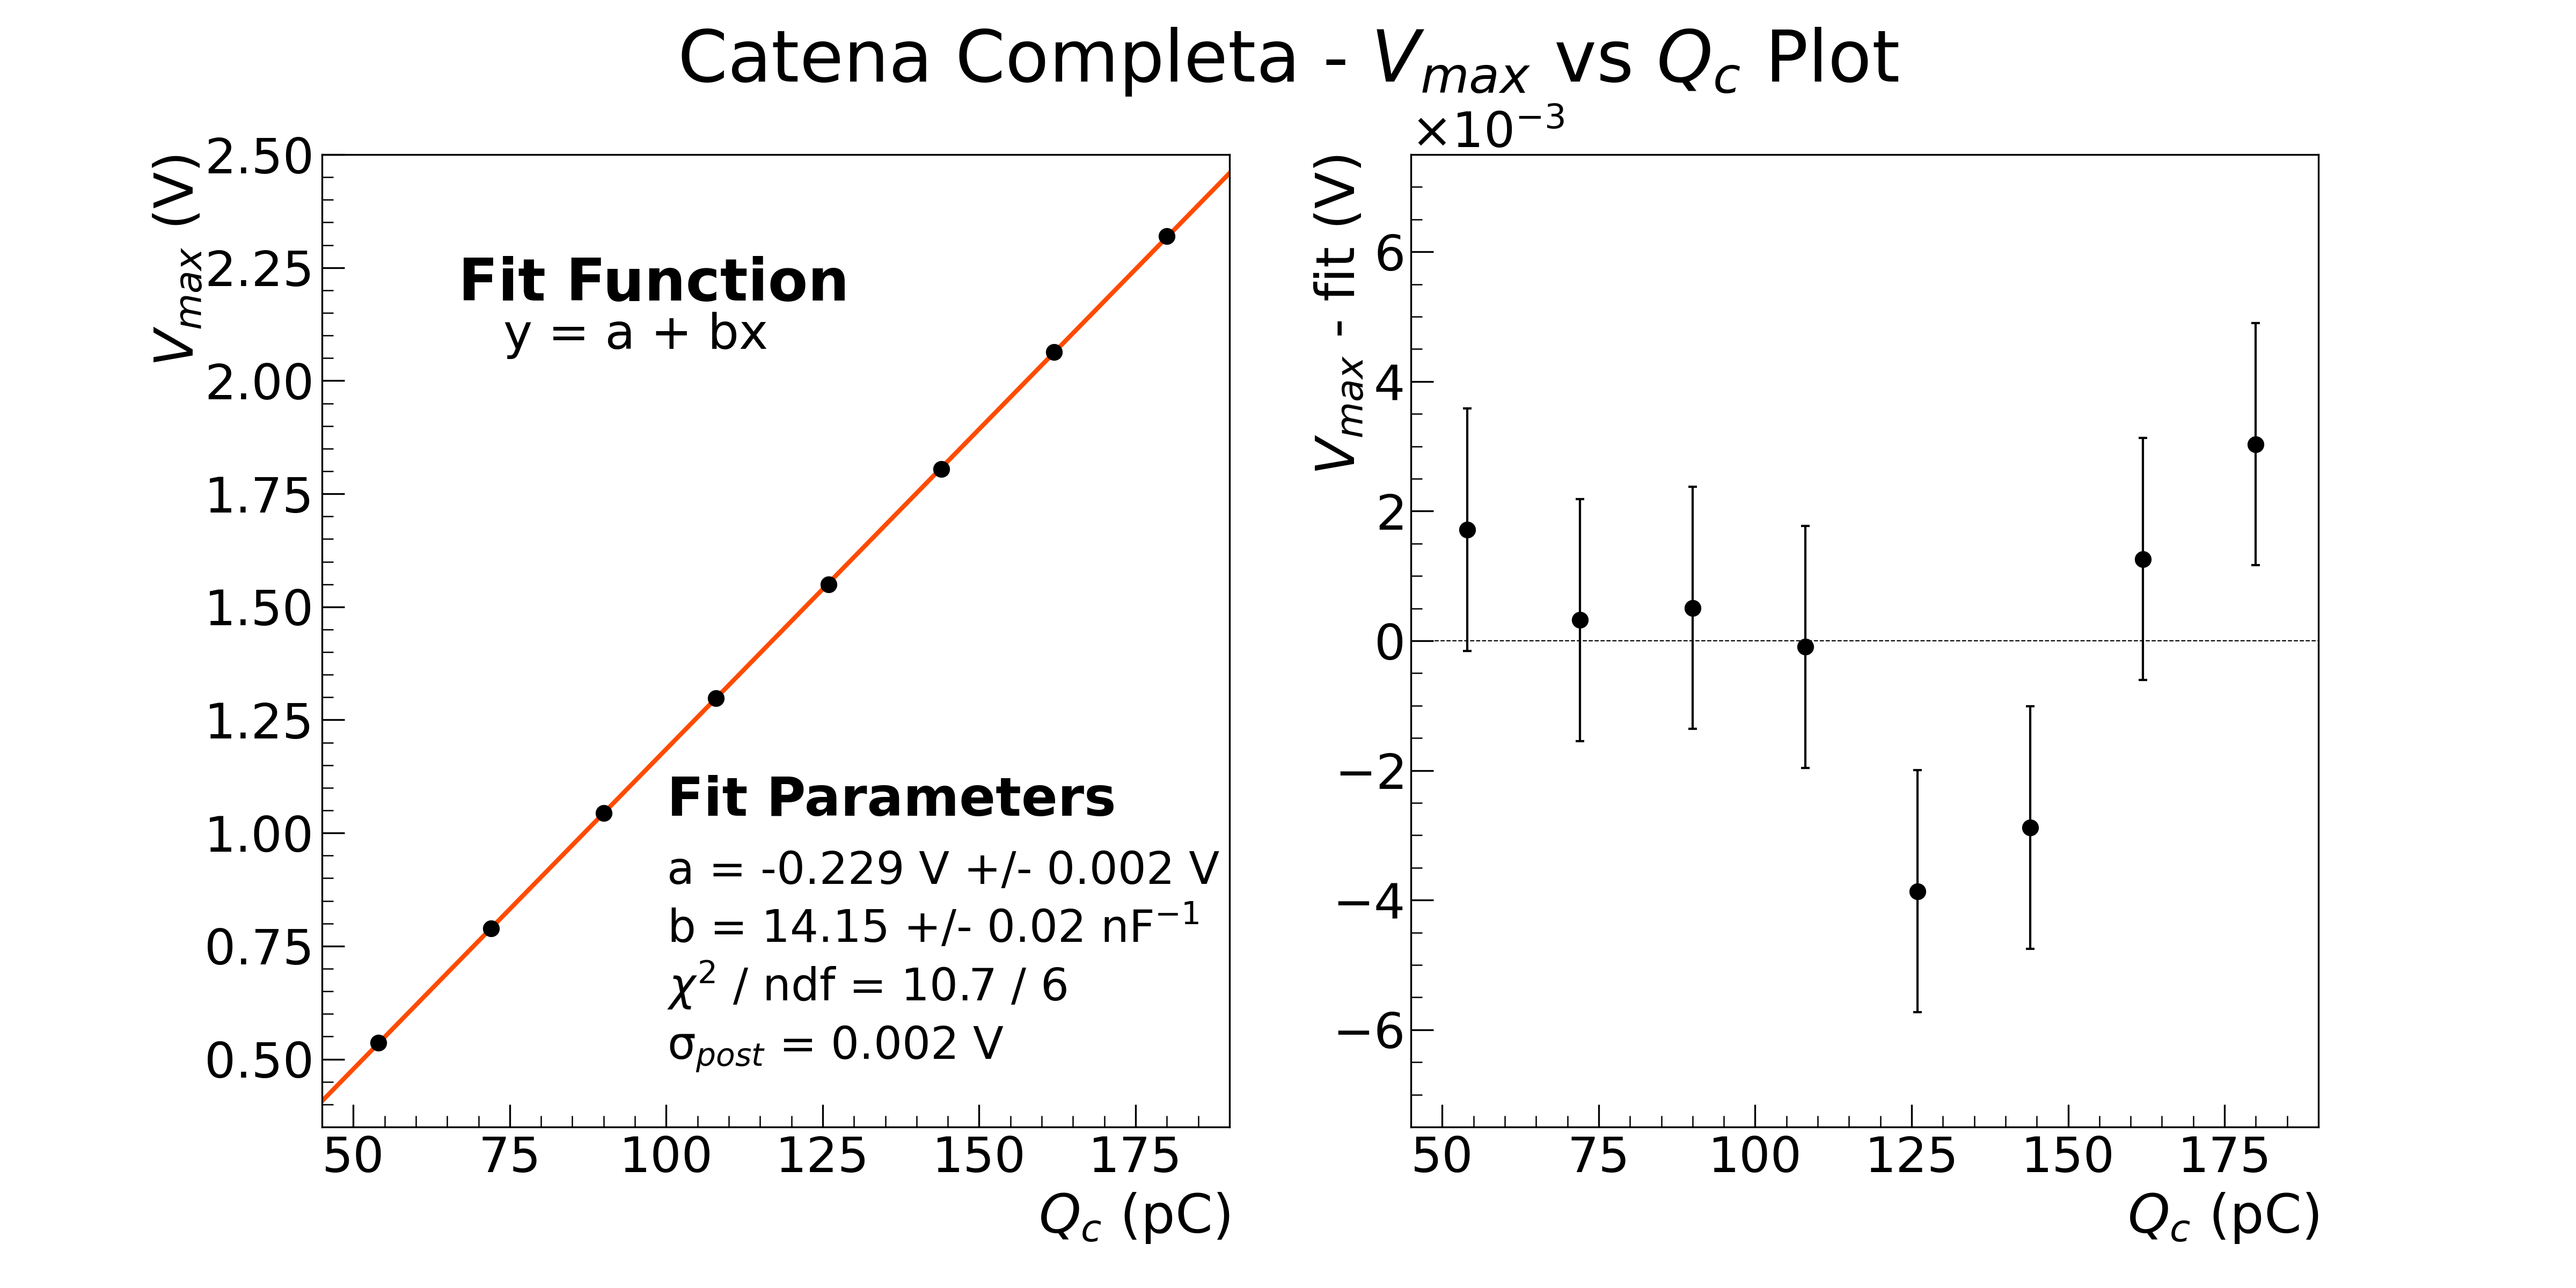
\includegraphics[width=0.9\linewidth]{../Plots/Catena/catena_linearity.png}
%\caption{\small Fit lineare del massimo di tensione in uscita contro la carica totale in ingresso.}
%\label{i:catena_linearity} \end{figure} \noindent Si nota immediatamente, osservando il grafico dei residui, come gli
%errori associati alle misure siano eccessivamente grandi a confronto con l'effettiva distribuzione dei punti attorno
%alla retta. Il $\chi^2$ infatti risulta essere molto minore rispetto al suo valore di aspettazione e l'errore a
%posteriori risulta essere circa un ordine di grandezza inferiore rispetto alle incertezze associate alle misure.
%L'andamento dei residui è sufficientemente regolare e, assieme all'ottima distribuzione delle misure attorno alla retta
%caratterizzata dall'errore a posteriori, si può quindi affermare una soddisfacente linearità della catena.\footnote{Si
%evidenzia che nel grafico in \autoref{i:catena_linearity} è stato reiettato il primo punto, corrispondente a
%$T=2\,\si{\us}$ in quanto fortemente fuori trend.}
%
%
%
%% 70.7 pF dal coefficiente angolare % 78.9968 pF dal parallelo C1 C2 shaper
%
%%-------------------------------------------------------------------------------------------------------------------------------------------
%%  THEBODE
%%-------------------------------------------------------------------------------------------------------------------------------------------
%
%\subsection{Analisi in Frequenza}\label{s:catena_bode}
%
%Si vuole ora studiare la risposta in frequenza della catena elettronica: si imposta il generatore in modo da erogare
%un'onda sinusoidale di ampiezza $1\,\si{\volt}$ e frequenza $f_{\text{gen}}$ variabile da $10\,\si{\Hz}$ a
%$100\,\si{\kilo\Hz}$. Per quanto riportato in \autoref{s:catena_config}, ci si aspetta un comportamento da filtro passa
%basso avente frequenza di taglio analoga a quella dello \textit{shaper} (\autoref{s:shaper_bode}). Si acquisisce quindi
%l'ampiezza del segnale sia in ingresso sia in uscita utilizzando l'oscilloscopio e viene calcolata la funzione di
%trasferimento $H$, alla quale viene associata un'incertezza $\sigma_{H}$ data da \autoref{e:preamp_H_err}. L'incertezza
%di guadagno associata all'oscilloscopio non viene invece considerata in quanto, dovendo successivamente prendere il
%logaritmo $\text{log}_{10}H$ della funzione di trasferimento, tale contributo viene scaricato interamente
%nell'intercetta delle interpolazioni volte a caratterizzare l'andamento delle misure. Si assume infine trascurabile
%l'incertezza sulla frequenza dell'onda erogata dal generatore. Si rappresenta allora in \autoref{i:shaper_thebode} il
%grafico di Bode delle misure acquisite assieme ai punti ottenuti attraverso una simulazione Spice della risposta del
%circuito (pagina seguente). Confrontando inizialmente le misure sperimentali con la simulazione Spice, si nota un
%ottimo accordo in tutto lo spettro di frequenze. Questo è chiaramente indice di una risposta in frequenza conforme alle
%aspettative: a basse frequenze la funzione di trasferimento è costante a $20.1 \pm 0.2 \,\text{dB}$ mentre per
%frequenze crescenti la funzione di trasferimento subisce un'attenuazione lineare di pendenza $-39.2\pm
%0.3\,\text{dB/dec}$, in linea con l'aspettativa dei $-40\,\text{dB/dec}$ dovuti al polo doppio. L'ascissa del punto di
%intersezione tra le due rette di regressione fornisce quindi una stima della frequenza di taglio del circuito
%$f_{\text{t}}= 9.72 \pm 0.13 \,\si{\kilo\Hz}$. Si ricorda quindi che la frequenza di taglio teorica attesa è
%$f_{\text{t}} = 10.0 \pm 0.4 \,\si{k\Hz}$, mentre la frequenza relativa al polo della funzione di trasferimento dello
%shaper ricavata dal grafico di Bode in \autoref{i:shaper_thebode} risulta essere $f_{\text{t}} = 9.6 \pm 0.2
%\,\si{k\Hz}$. La stima della frequenza di taglio appena trovata presenta un'ottima compatibilità con queste ultime: in
%particolare si ha una compatibilità $\lambda = 0.7$ con la stima teorica e $\lambda = 0.3$ con la frequenza relativa al
%polo dello \textit{shaper}. \begin{figure}[H] \centering
%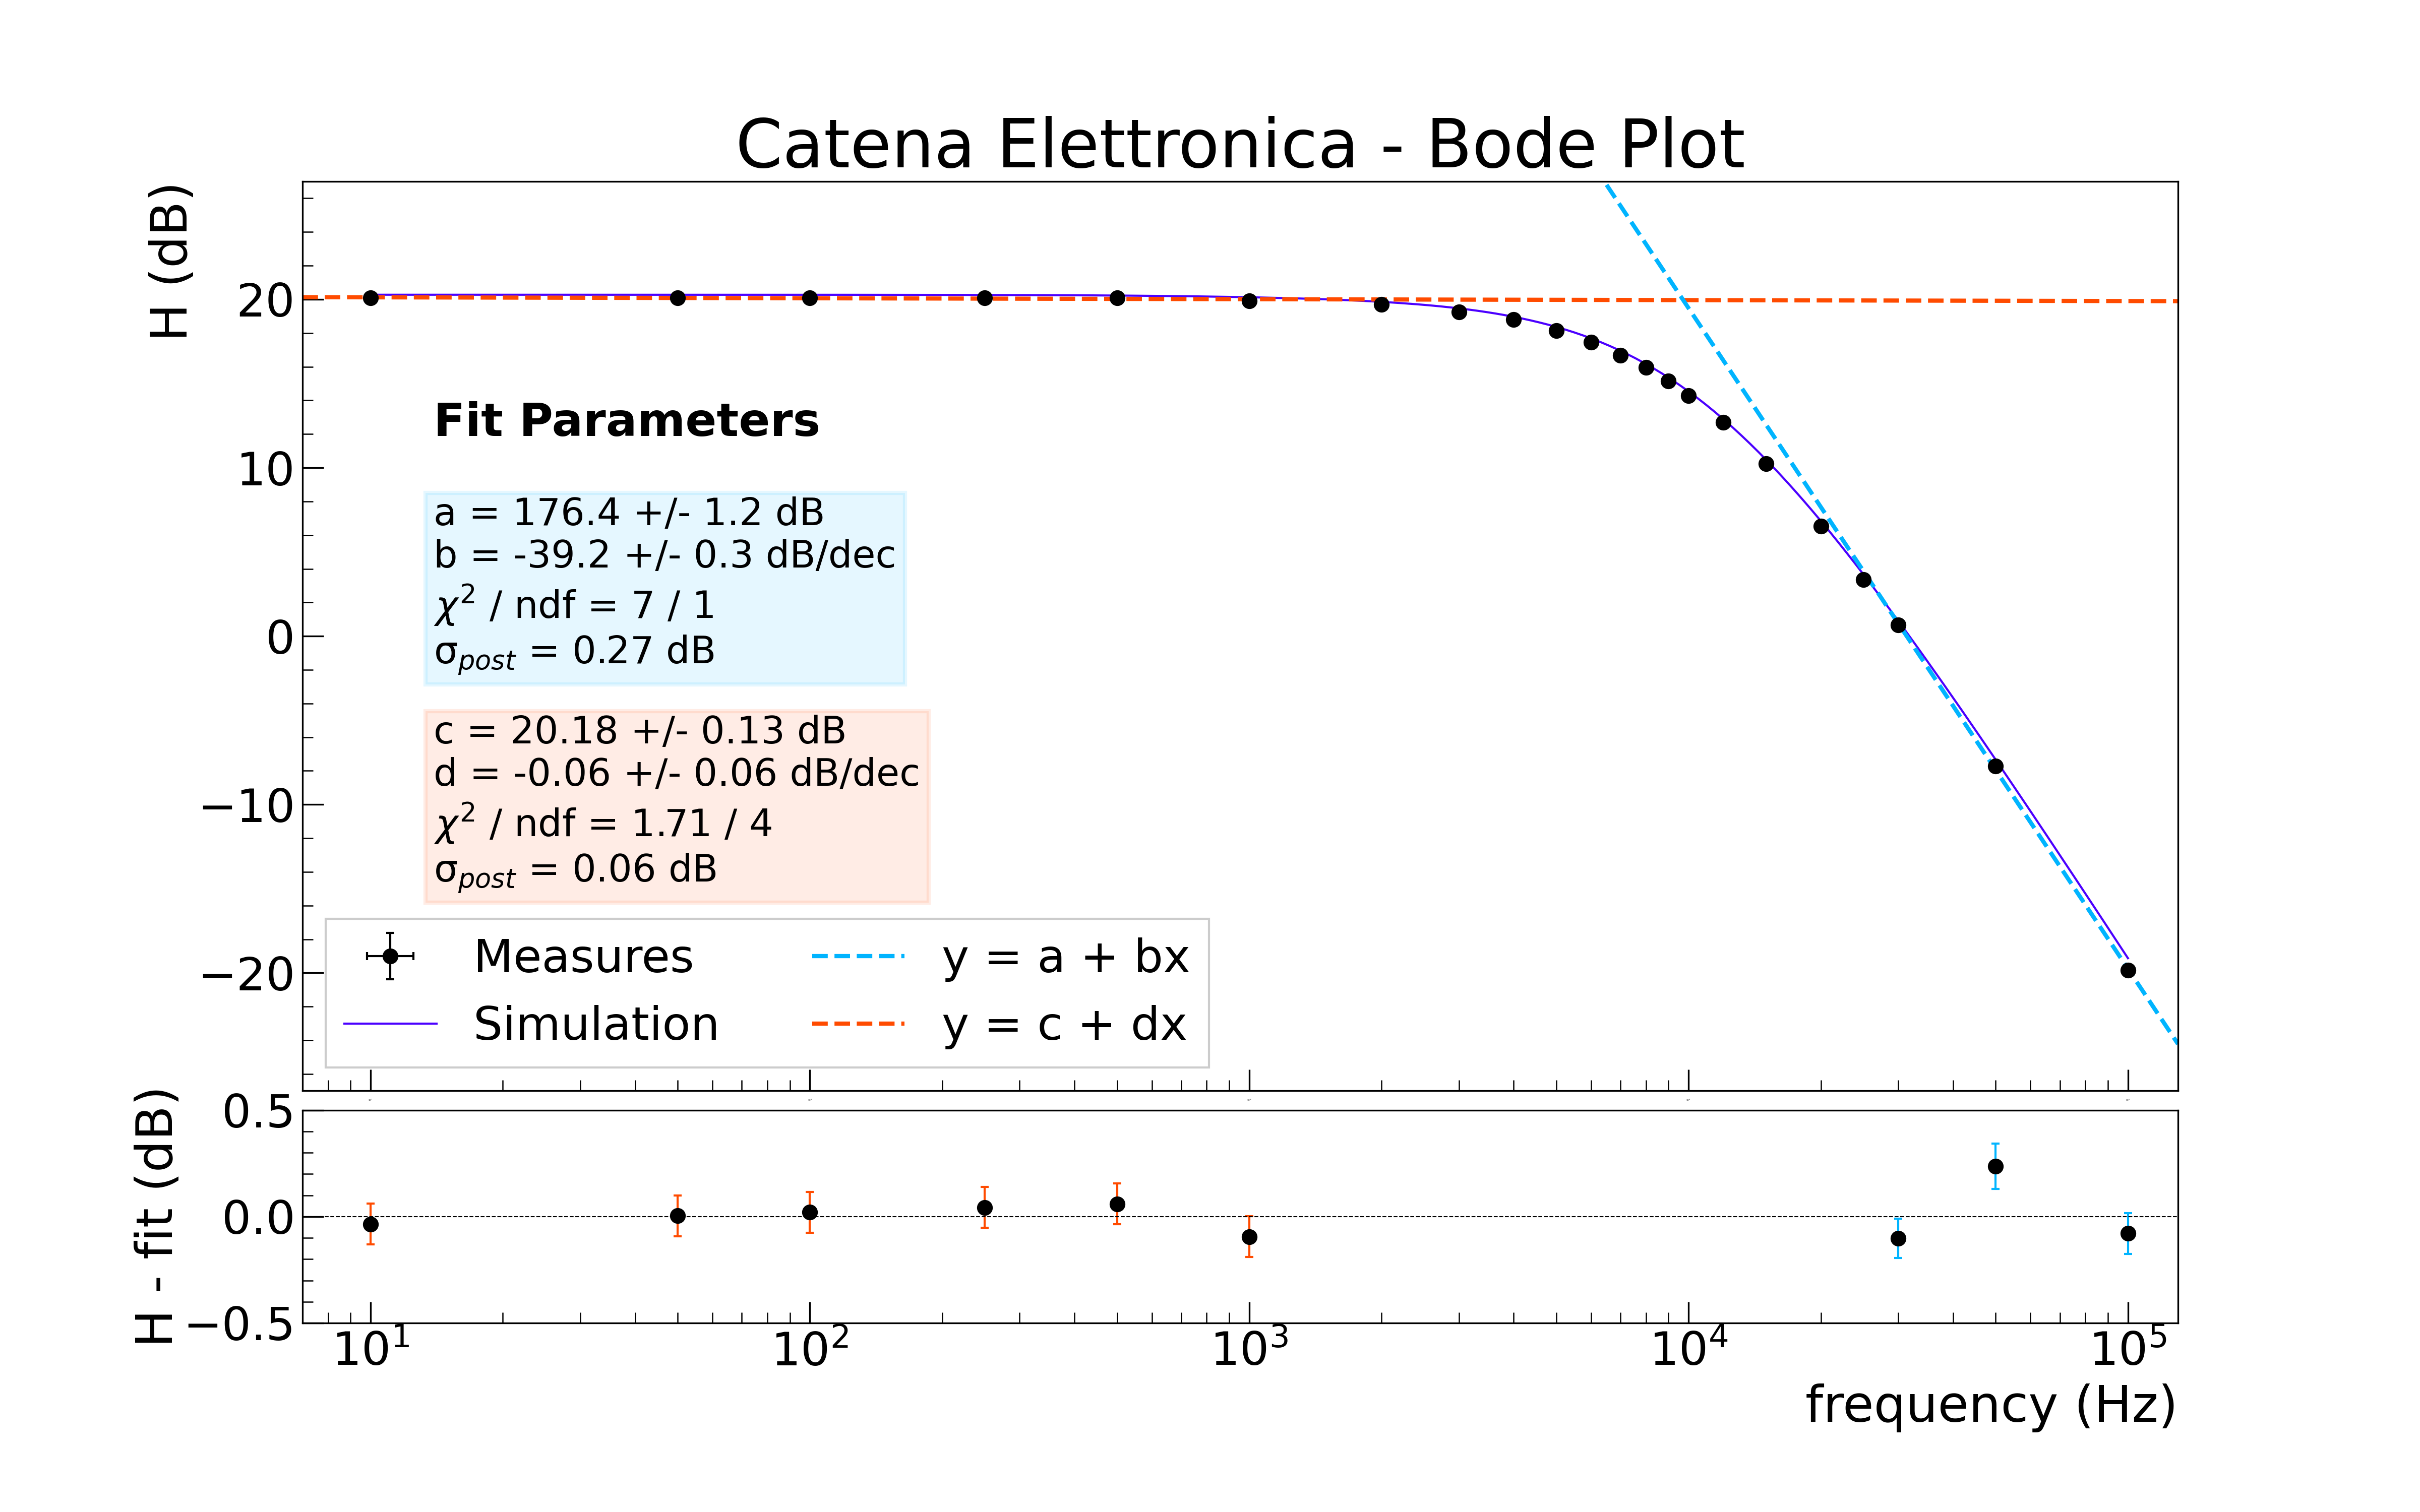
\includegraphics[width=0.9\linewidth]{../Plots/Catena/bode_plot.png} \caption{\small Grafico di Bode delle misure
%sperimentali e dei dati simulati.} \label{i:catena_thebode} \end{figure} \noindent È stata quindi verificata la
%validità di \autoref{e:catena_H_final}, fortemente dipendente dalla corretta scelta delle componenti circuitali al fine
%di poter effettuare determinate approssimazioni e identificazioni. 























%----------------------------------------------------END OF FILE----------------------------------------------------------------------------
\end{document}